


        
        \section{Neutron stars in binary systems}
        \label{binary_NS}

Continuous waves from neutron stars in binary systems are doubly distinctive.
As Section~\ref{continuous_waves} comments, binary systems constitute perhaps a substantial fraction (see the ATNF catalog~\cite{ManchesterATNF2005}), perhaps half, of continuous wave (CW) sources.
CW search methods prove both powerful, probing well below the LIGO amplitude spectral density (ASD) noise floor given year-length science runs, and computationally-demanding.
Taken together, a non-trivial possibility exists that there are CW from neutron stars (NS) in binary systems, buried in existing or forthcoming data, that could be seen with a fast, tractable search method.

TwoSpect~\cite{GoetzThesis,GoetzTwoSpectMethods2011,GoetzTwoSpectResults2014} is such a method. 
Developed as a search for pulsars in binary systems with unknown sky location, orbital period, projected semi-major axis or frequency, it has been tested and run on S6 data.
In such a mode it accepts some degradation of sensitivity in order to scan the entire parameter space.
If some parameters are known, a deeper search becomes possible.
This chapter describes the development of this `directed' search and its application to a simulated data set (a `Mock Data Challenge' or MDC).
The next chapter elaborates the results when applied to data from the last science run, S6.

            %Astrophysical prospects for binary pulsar detection. 
            %Binary pulsars are perhaps our best hope for detecting continuous gravitational waves.

%\begin{frame}{Neutron stars in binary systems}
\subsection{Continuous gravitational waves from neutron stars}
%\begin{definition}
%Neutron star with a partner in a binary system, 
%e.g., a low-mass X-ray binary (LMXB)\end{definition}

%\begin{example}
%Scorpius X-1
%\end{example}

Choosing to pursue binary sources is itself a choice of search direction.
Neutron stars can be in isolated systems as well, for which many searches have been conducted (summarized in Section~\ref{continuous_waves}).
Yet isolated stars have several issues that make them challenging to detect.
Isolated stars have a finite lifetime (albeit many millions of years) over which they are hypothesized to emit detectable GWSs.
During this detectable lifetime, they are losing energy to GWs -- this energy loss results in a continually-slowing frequency, denoted by the spindown rate $\dot{f} = df /dt$.
Spindown in turn makes GW searches more computationally challenging: templated-phase mismatch over a science run of many months is often significant enough to require additional templates to search over putative spindown values. 
Since many searches are already computationally limited, a GW source without these challenges would arouse interest.

Binary systems generate such interest.
LMXBs, low-mass X-ray binaries, of which Scorpius X-1 (Sco X-1) is typical, are at the focus.
As understood from the work of Papaloizou \& Pringle~\cite{PapaloizouPringle1978} and Wagoner~\cite{Wagoner1984}, LMXBs might exhibit several key properties:

\begin{itemize}
\item Longer lifetime than isolated sources, due to accretion recycling
\item Ellipticity \& hot spots, due to accretion
\item Hypothetical \textit{torque balance} frequencies
\end{itemize}

Not only are LMXBs an abundant fraction of the neutron star population, they also constitute a disproportionate quantity of fast period, \textit{millisecond} pulsars -- and interestingly may be capped at a speed limit (hypothesized by Chakrabarty~\cite{Chakrabarty2003}) below the relativistic breakup limit.
If so, LMXBs in particular would constitute an ideal search target.
Let us review the points of lifetime, ellipticity, and torque balance in further detail.

%Potential candidates for gravitational waves:
%\begin{itemize}
%\item Longer lifetime than isolated sources (recycling)
%\item Ellipticity \& hot spots due to accretion
%\item Torque balance hypothesis (Papaloizou \& Pringle 1978, Wagoner 1984):
%\item \emph{bright ms pulsars}
%\item Speed limit? (Chakrabarty 2003)
%\end{itemize}
%\end{frame}


            \subsection{Binary spin-up and detectable lifetime}
            \label{spin-up}
         
                %GW pulsar lifetime alone vs companion.
As stated, isolated, elliptical, rotating NS will lose energy to GW.
This intrinsically makes their interesting GW radiation short-lived.
Binary systems, in contrast, can be recycled by accretion.
Not necessarily a steady process, recycling of infalling matter from an orbital partner can raise the spin frequency of a neutron star by conservation of angular momentum.
Energy is released as heat and radiation on impact with the surface of the NS, in particular as X-rays in the case of an LMXB.
The work of Papaloizou, Pringle and Wagoner elucidates the implications for GW detection.
As infalling matter hits an NS, the matter stream can not only increase the spin frequency -- and thus GW radiation amplitude -- of the NS, but it can also increase ellipticity at the hot spot.
Equation~\ref{cw_radiation_eps_eq} shows that this further increases radiated GW ampltitude.
Insofar as the infall stream continues, the NS can be `spun-up' to rotation frequencies with non-negligible GW emission, potentially for a far longer detectable lifetime than an isolated star.

Spin-up might proceed, as Wagoner in particular derives, only up to a specific frequency.
In this \textit{torque balance} hypothesis, the matter infall delivers a torque offset by GW emission; since GW emission rises with frequency squared, an NS that is spinning up due to accretion will eventually reach a limiting frequency beyond which GW emission prevents it from spinning faster.
This idea connectis accretion rate with GW emission.
Since accretion rate can be measured electromagnetically, in X-ray flux $F_\times$, this lets us estimate what level of GW emission could be expected for a star rotating at frequency $\nu$ (Equation~\ref{torque_bal_eq}): 

\begin{equation}
h_{0}=5\times10^{-27}\left(\frac{300\textup{Hz}}{\nu}\right)^{1/2}\left(\frac{F_{\times}}{10^{-8}\textup{erg cm}^{-2}\textup{s}^{-1}}\right)^{1/2}.
\label{torque_bal_eq}
\end{equation}

\noindent Torque-balanced neutron stars would remain at their torque-balance frequency: accretion would counteract spindown.
This frequency stationarity is computationally useful.

            \subsection{Detection rate projections}
            \label{rate_projections}

                %aLIGO rate projections.
Equation~\ref{torque_bal_eq} is incentive to develop searches especially for LMXBs.
Although the predicted $h_0$ is still low, it is conceivable that high-luminosity such as Scorpius X-1 (see Section~\ref{scox1_parameters} for full parameters) might just be within reach of advanced detectors such as aLIGO.
Unknown sources with potentially higher GW luminosity, perhaps with X-ray flux not directed toward our solar system, are a motivation for making this search capable of scanning the entire sky.
It is difficult to infer how many sources might exist, but over 50 accretion-powered X-ray pulsars were already known as of 2005~\cite{ManchesterATNF2005}.
Known, especially-promising sources such as Scorpius X-1 warrant scrutiny with a deeper, \textit{directed search} over their known parameter space.
Such searches are the purpose of TwoSpect.

        \section{TwoSpect searches}
        \label{all-sky}

TwoSpect offers a way to calculate a statistic and infer detection probability for a putative template waveform of a neutron star emitting continuous GW in a binary system.
LIGO CW searches generally use matched filters, like inspiral searches. 
Although the filter is easier than the inspiral waveform to calculate, the net computational cost is much higher, since integration covers a longer timespan, compensating for weaker signals. 
Matched filtering a binary pulsar search in the time-domain, with complete phase information, appears be computationally intractable for terascale computer clusters in the early 2010s. 
By switching the problem to frequency domain power instead of amplitude, the search becomes feasible, albeit at a cost in sensitivity.

TwoSpect performs two transforms: it first parcels a science run (year-scale) into overlapping short Fourier Transforms (SFTs, hour-scale or less).
SFT frequency bins for a given data stretch are then adjusted to the frequency at the solar system barycenter, accounting for Doppler shifting that would be induced at the sky location, frequency, and time under investigation.
Each row of constant-barycentered frequency bins is then treated as a time series.
That time series is then Fourier transformed too -- the two in TwoSpect.
This transformed yields a plane of pixels: the frequency-prime $f'$ vs frequency $f$ plane.
Goetz~\cite{GoetzThesis} developed this technique in the context of GW.
The plane of pixels provides a tractable data set on which binary CW templates can be tested.

Detectable strain $h$ scales poorly with time, $T^{1/4}$, due to the double transform, instead of $T^{1/2}$ for a coherent search, but matched templating techniques are powerful enough that being able to use them is promising.
Goetz developed a noise-subtracted $R$-statistic to measure the cumulative power in each binary CW template.
This statistic follows a distribution as the sum of many $\chi$-squared distributions (see Taylor~\cite{taylor} as well as Casella and Berger~\cite{CasellaBerger2001} for statistical reference) and yields consistent $p$-values.
These $p$-values can be extrapolated from Davies' method, having been vetted by Monte Carlo~\cite{GoetzTwoSpectMethods2011}.
By providing these statistics, TwoSpect yields information on a large fraction of parameter space heretofor unsearchable.
The code is open source and available online~\cite{LALAPPSrepo}.

%            TwoSpect methods as-is. These are described in detail in Evan Goetz's thesis~\cite{GoetzThesis}. %Note that the code is located on the web freely accessible in the LALApps repository~\cite{LALAPPSrepo}.

%For primers on error analysis and statistics, see Taylor~\cite{taylor} as well as Casella and Berger~\cite{Ca%sellaBerger2001}.

            \subsection{Two spectra: a double Fourier transform}
            \label{two_spectra}

       %         'Two spectra' -- FFT of periodograms reveals modulation of sine waves.

The double-Fourier transform is illustrated in Figures~\ref{tfplane-figure} and~\ref{ffplane-figure}.
Existing LIGO routines perform the steps needed to generate the first figure: SFTs are made in pre-processing and then barycentered.
TwoSpect then re-invokes the Fast Fourier Transform routines to transform the frequency vs time plane into a frequency vs frequency-prime plane.
Although GW phase information is lost (and, for now, templates ignore orbital phase), the resulting search domain is robust against spin wandering.

\begin{figure}
\begin{center}
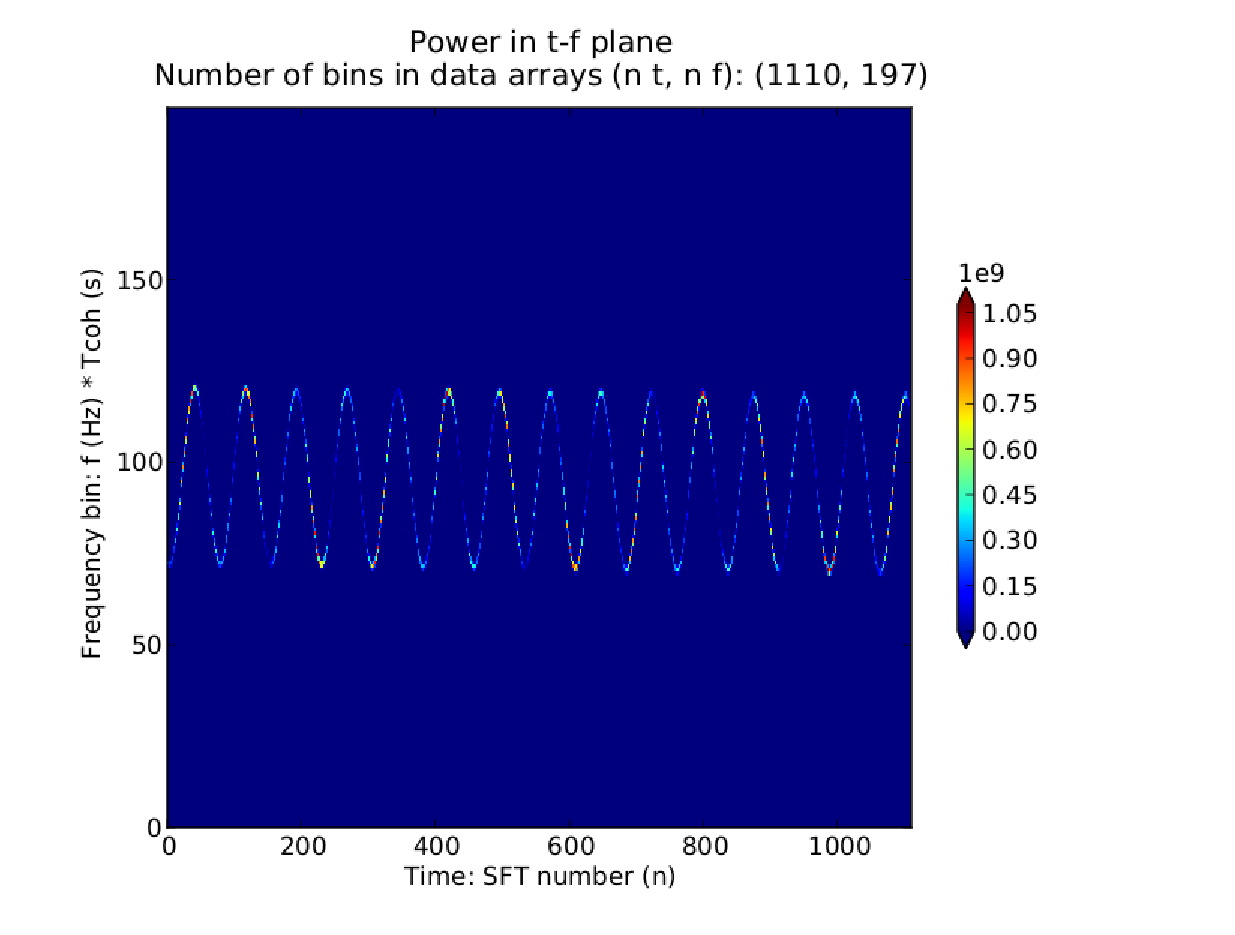
\includegraphics[width=0.8\paperwidth,height=0.4\paperheight]{tfplane-4e21-on-4e24.eps}
\caption{After Doppler-shifting the frequencies into the solar system barycenter, TwoSpect analyses begin on this first, time-frequency plane. A simulated signal at 100.015 Hz and $\textup{asini} = 1.44$ is injected with $h_0 = 4\times 10^{-21}$ into $10^6$ seconds of Gaussian noise at $Sh = 4 \times 10^{-24}$ (the projected minimum Advanced LIGO noise level); the signal period is 68023.8259 seconds, as with Scorpius X-1.}
\label{tfplane-figure}
\end{center}
\end{figure}

\begin{figure}
\begin{center}
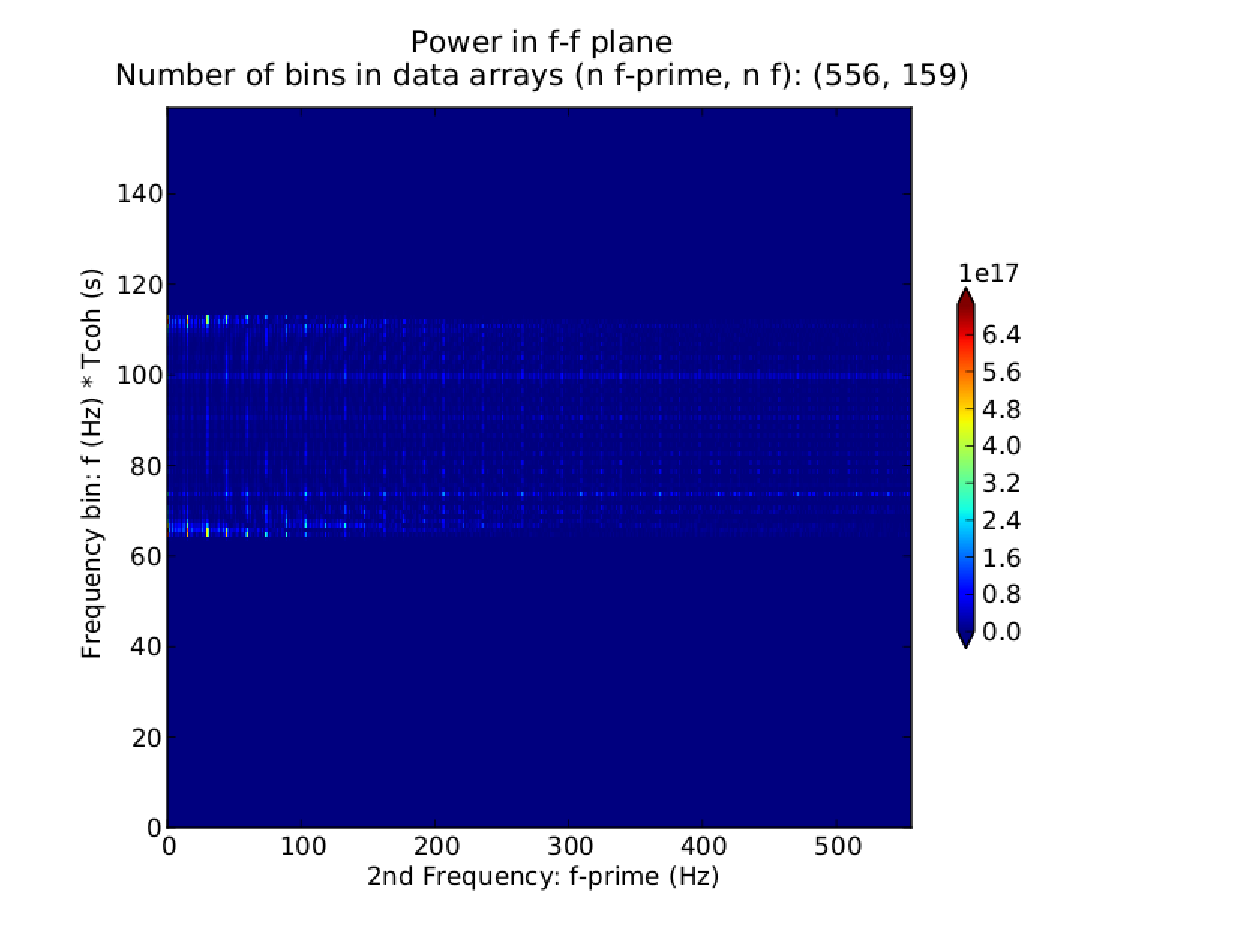
\includegraphics[width=0.8\paperwidth,height=0.4\paperheight]{ffplane-4e21-on-4e24.eps}
\caption{Fourier-transforming along the `rows' (constant frequency bin, variable time bin) generate a second plane, the frequency-frequency plane. The power of each bin in this transform is plotted as a pixel. By aggregating power, this second Fourier transform enhances signal so that matched templates can be applied for a search.}
\label{ffplane-figure}
\end{center}
\end{figure}

            \subsection{Infering neutron stars with companions}
            \label{inference}
 
                %Infer whether modulation is due to a companion star.
With the search domain prepared, templates can be tested.
The modulation induced by LMXB partners on their NS companions is typically fractions of a Hertz.
Modulation depth is, more precisely~\cite{GoetzTwoSpectMethods2011},

\begin{equation}
\Delta f = \frac{2 \pi f (a \sin i)}{P},
\label{TwoSpect_mod_depth}
\end{equation}

\noindent where in $f$ is GW emission frequency, $a \sin i$ is projected semi-major axis, and $P$ is orbital period.
Equation~\ref{TwoSpect_mod_depth} specifies the amplitude of the sinusoid seen in Figure~\ref{tfplane-figure}, though it must be noted again that it is the power of the transform of that sinusoid in Figure~\ref{ffplane-figure} that is actually template-tested.


%\begin{frame}{TwoSpect algorithm for all-sky binary searches}
\subsection{TwoSpect algorithm detection statistic}

%TwoSpect (Goetz \& Riles 2011), supplied this  searches for patterns in
%doubly Fourier-transformed data from binary's orbital modulation
%\emph{doubly Fourier-transformed:} $k$ frequency bins, time series
%$n$
%Short Fourier Transform series, along $n$, is FFT'd 

Template-testing proceeds from a given test frequency $f$, modulation depth $\Delta f$ (via astrophysical $a \sin i$), and period $P$ using data prepared for some sky location. Having a time series $n$ SFTs long with $k$ frequency bins, a template weight can be computated for a number of pixels $M < n*k$.
Applying these weights yields the $R$-statistic:

\begin{equation}
R=\frac{\Sigma_{i=0}^{M-1}w(m_{i})[Z(m_{i})-\lambda(m_{i})]}{\Sigma_{i=0}^{M-1}[w(m_{i})]^{2}},
\label{TwoSpect_R_statistic}
\end{equation}

\noindent where
\begin{itemize}
\item $R$: template detection statistic
\item $w$: template weight
\item $i$: pixel index of $M$ pixels
\item $Z$: spectral power (after barycentric correction)
\item $\lambda$: expected noise power
\end{itemize}
%$\rightarrow$ E. Goetz wrote, conducting all-sky search
%\end{frame}
% Everything below is imported from my APS and AEI talks (harmonized)

\begin{figure}
\begin{center}
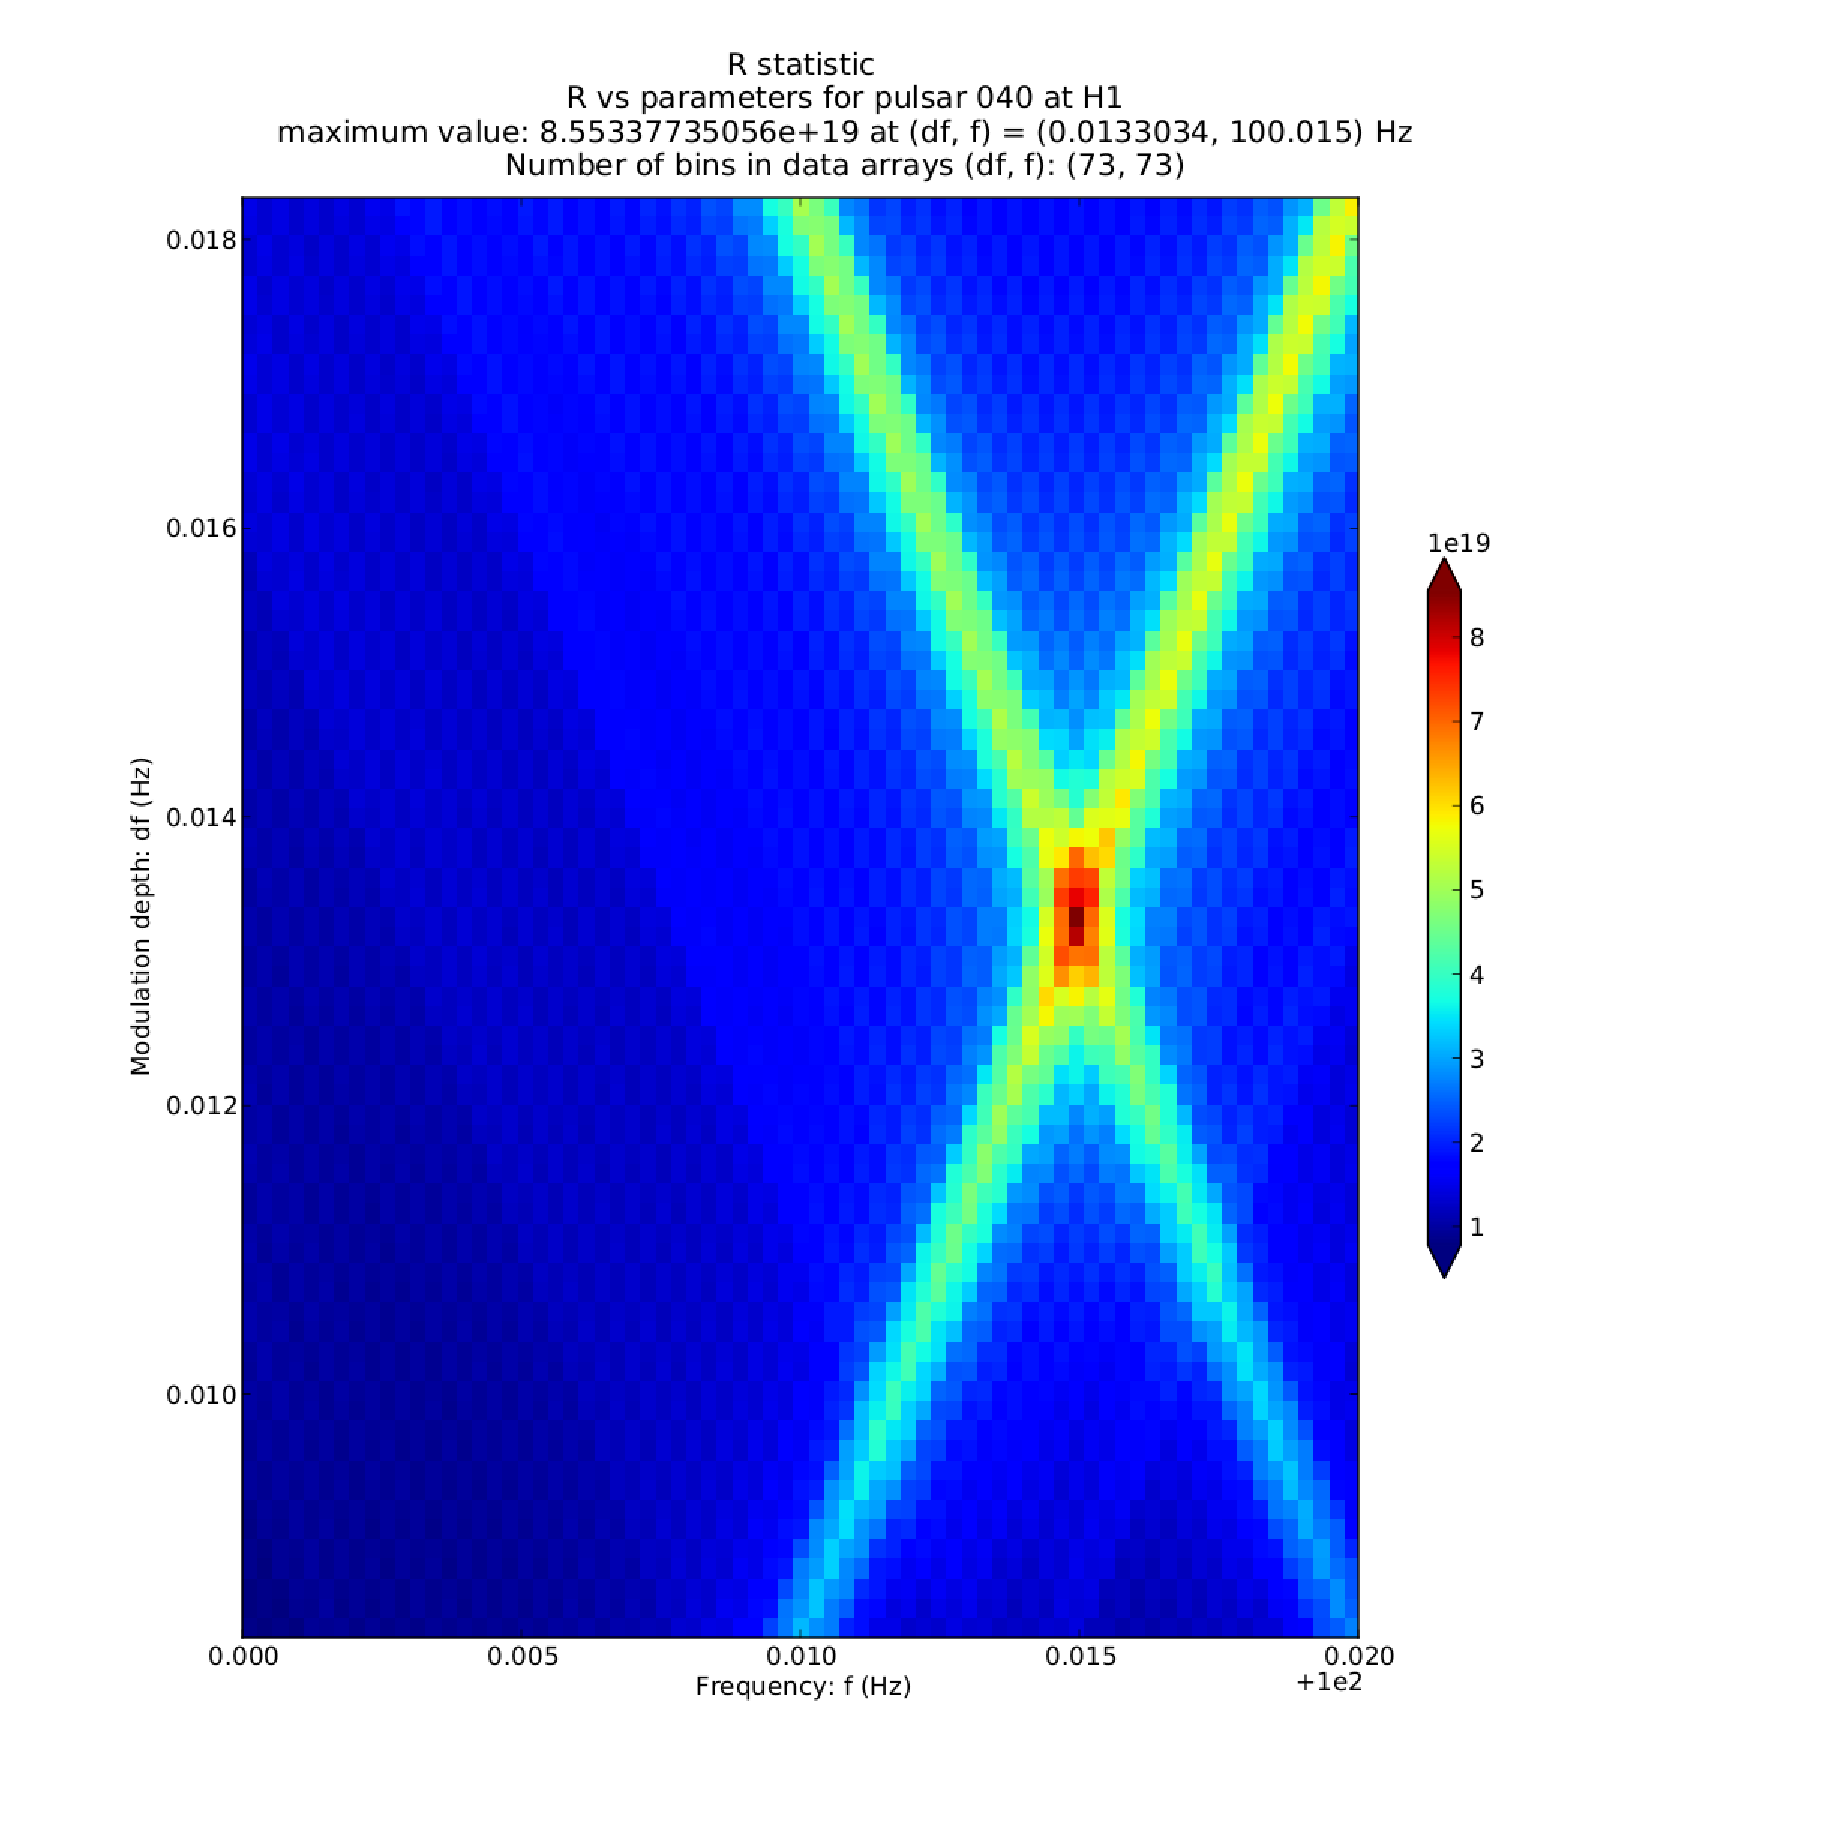
\includegraphics[width=0.8\paperwidth,height=0.62\paperheight]{R-4e21-on-4e24.eps}
\caption{Exact templates for putative singals weight the pixels in the frequency-frequency plane to generate $R$ statistic for a simulated pulsar (note: not the same as pulsar $40$ in the Scorpius X-1 mock data challenge) at 100.015 Hz and $\textup{asini} = 1.44$. The resulting $R$ values are heatmap-plotted on the modulation depth vs frequency plane.}
\label{inj_R_statistic}
\end{center}
\end{figure}

\begin{figure}
\begin{center}
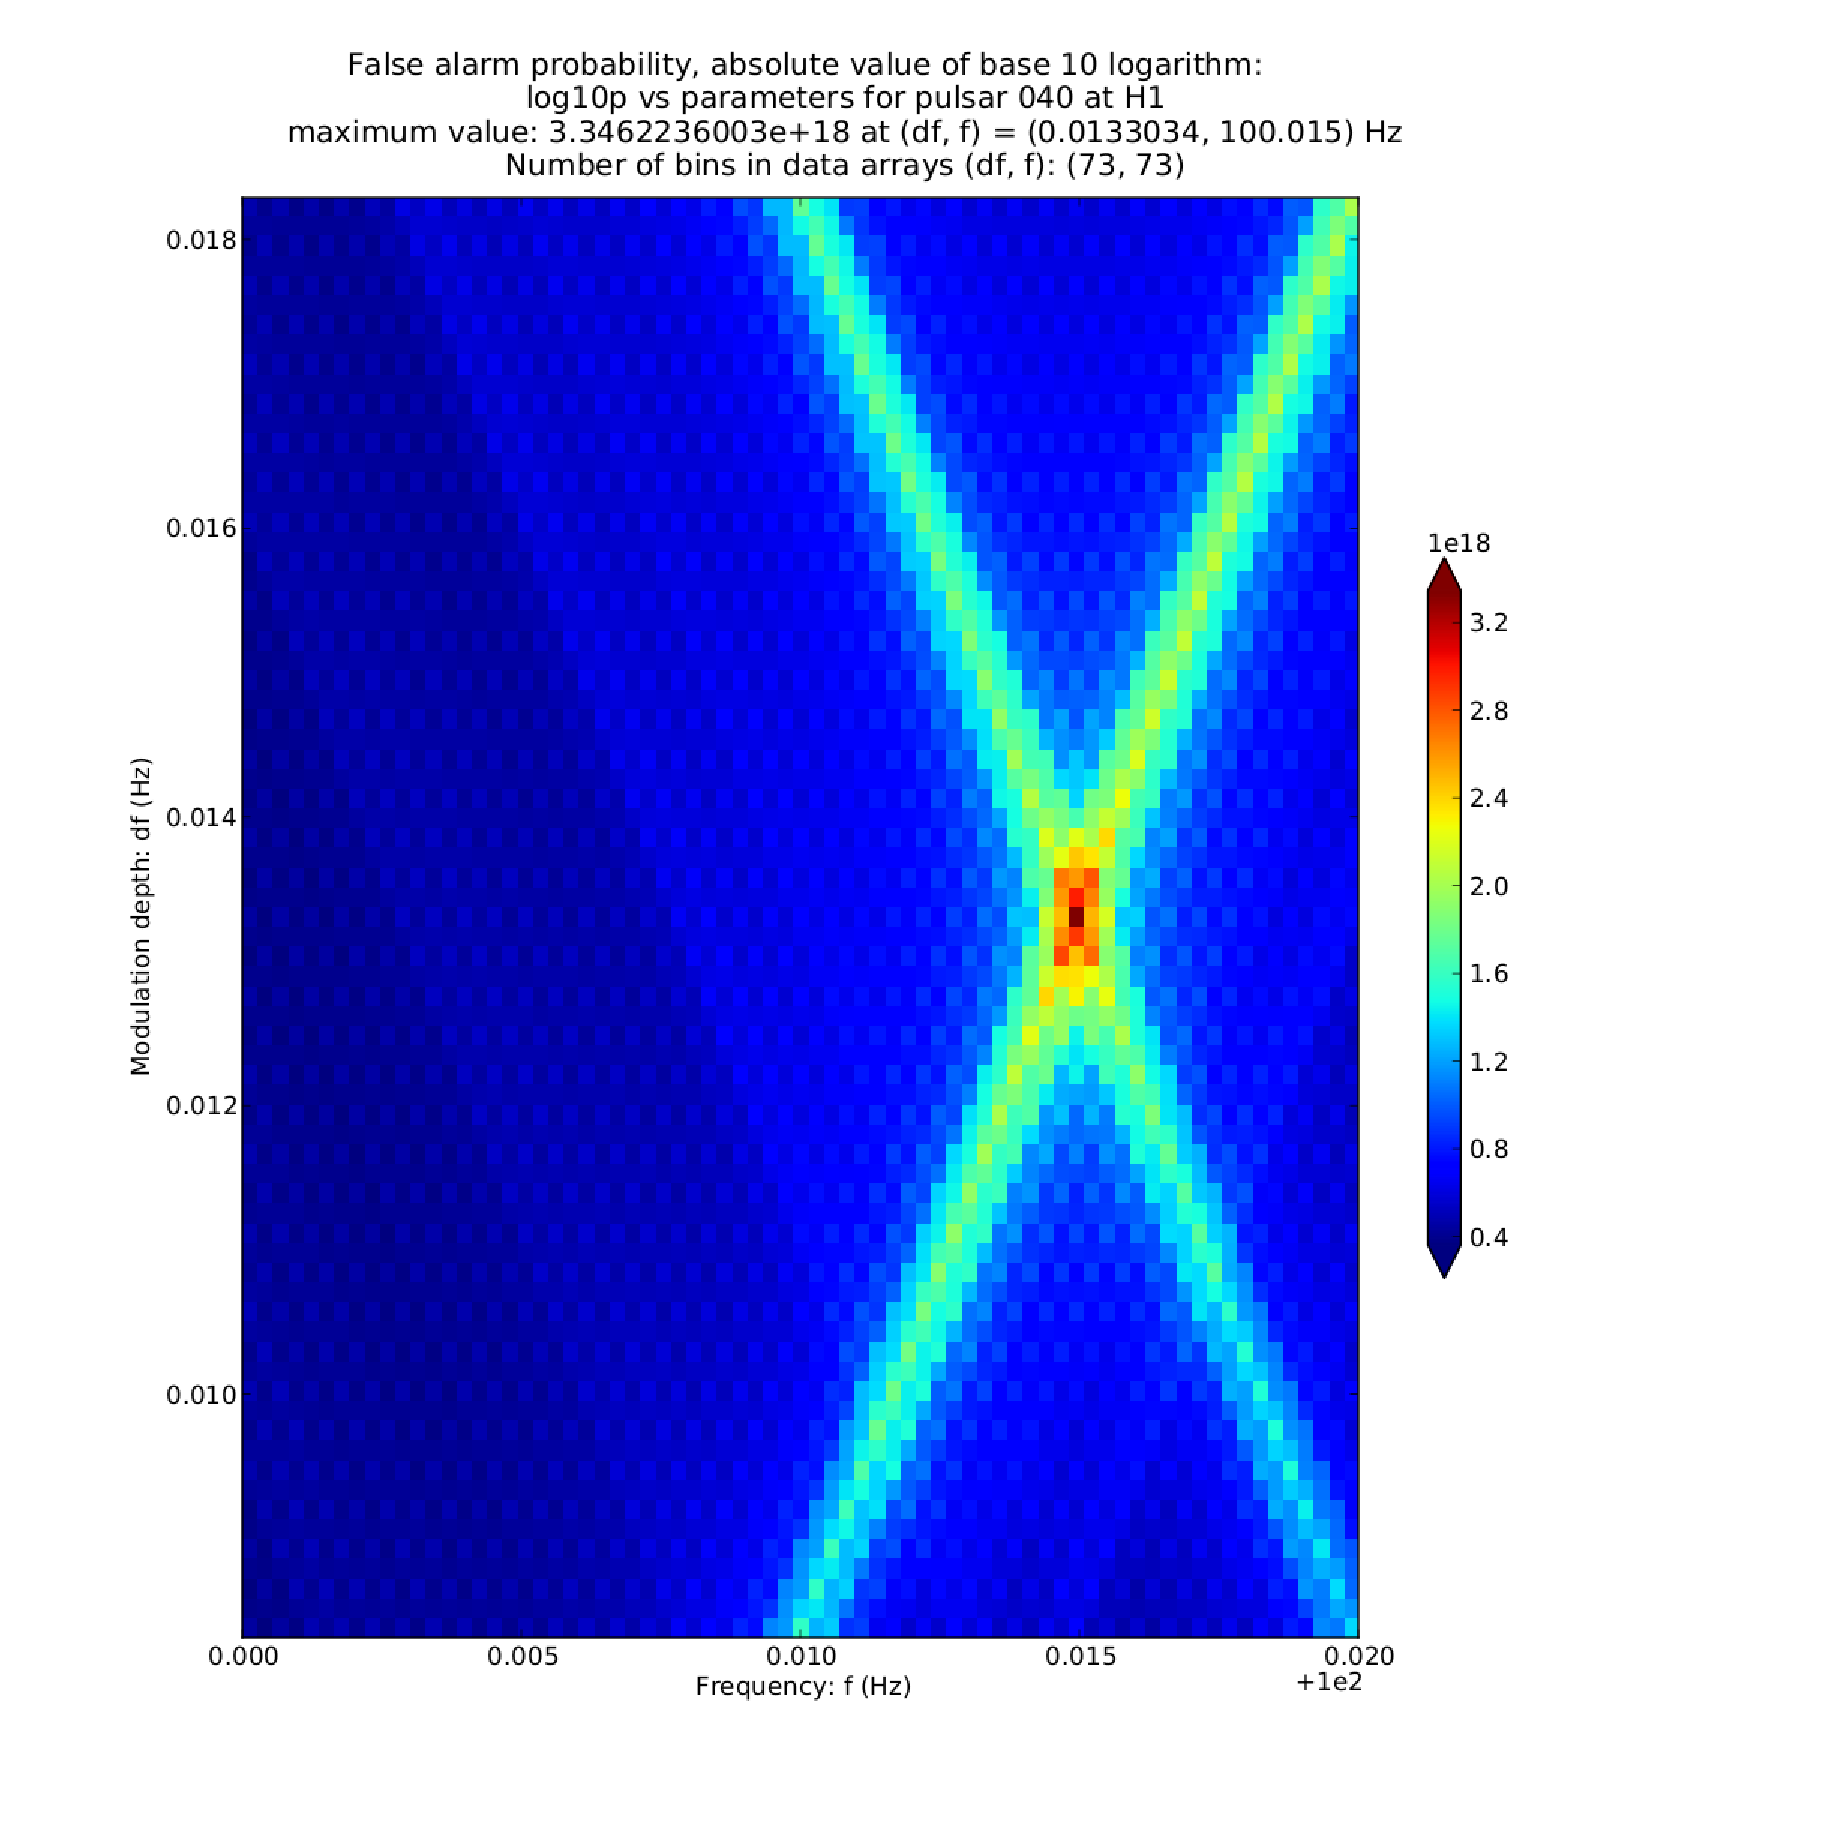
\includegraphics[width=0.8\paperwidth,height=0.62\paperheight]{Prob-4e21-on-4e24.eps}
\caption{The Davies algorithm translates $R$ statistic values for exact templates into (single-template) $p$-values, plotted on the modulation depth vs frequency plane.}
\label{inj_log10p}
\end{center}
\end{figure}

Testing various template models against simulated neutron stars in binary systems shows the value of $R$-statistic.
Figure~\ref{inj_R_statistic} shows that the statistic responds markedly when the input template values match the simulated `injection' sufficiently well.
The sharp response assures accurate parameter estimation.
Furthermore, Monte Carlo simulations by Goetz quantify the probability of high $R$ statistics arising in noise.
Using generating functions and Davies' method, this probability has already been incorporated into a single-template $p$-value, seen in figure~\ref{inj_log10p}.
Further, multi-trial Monte Carlo studies done by the author have validated the probability of $R$- and $p$-values arising in noise.


%\end{frame}

%\section{Directed searches for neutron stars in binary systems}

%\begin{frame}{Directed TwoSpect's greater sensitivity}
\section{Directed TwoSpect's greater sensitivity}

Searching over a wide range of right ascension and declination\footnote{Right ascension and declination date from at least the time of Ptolemy's \textit{Almagest} and are familiar in modern form in Copernicus's \textit{De revolutionibus orbium coelestium}~\cite{Hawking2002}. While ecliptic or more modern galactic coordinates can also be used, terrestrial Doppler motion is significant for CW searches and is most easily calculated in RA \& Dec.} can multiply computational times for gravitational wave searches by many orders of magnitude.
Each frequency GW needs to be corrected by a phase and amplitude Doppler correction unique to each sky location.
%Historical interest: the system of right ascension and declination were fixed by the time of Corpernicus, \textit{De revolutionibus orbium coelestium}~\cite{Hawking2002}.
The number of distinct sky points needed is discretized by the allowed mismatch in sensitivity between points.
Typically, we search over the parameter space with a grid that allows $0.2$ mismatch in $R$ statistic; the space is smooth enough that this grid can be smooth and rectangular.
Looking across all LIGO frequencies requires over $10^{18}$ templates, of order $\mathcal{O}(10^9)$ more templates~\cite{GoetzTwoSpectMethods2011} to do an all-sky analysis than a search at a single location and known period.
Thus the all-sky search is, in practice, only feasible when the $R$-statistic is the last in a stage of hierarchical statistics for candidate GW signals.
The initial stage of this hierarchy, an incoherent harmonic sum, is known~\cite{GoetzTwoSpectMethods2011} to reduce potential sensitivity.

A \textit{directed} search could be narrowly focused enough to calculate $R$-statistics for all interesting binary CW models at a particular point in parameter space.
%There are several reasons to pursue more \textit{directed} searches in addition to the all-sky search.
With a known electromagnetic counterpart, such as an LMXB or X-ray transient (XTE), the parameter space can often be reduced to a particular sky location (known to a few milliradians or better) and period (known to fractions of a second).
Frequency may (as with XTE J1751-305~\cite{Markwardt2002}) or may not (as with Scorpius X-1~\cite{Galloway2014}) be known\footnote{It may be noteworthy at our 8.5 kiloparsec galactic radius~\cite{KerrLyndenBell1986} that both these sources are located in the direction of the galactic center.}.
%\emph{All-sky search: }parameter space $\gg10^{18}$ templates
%\begin{itemize}
%\item Hierachical search; incoherent harmonic sum to consolidate\\
%parameter space, use templates to test interesting outliers
%\end{itemize}
%\emph{Directed search: }parameter space much smaller
%\begin{itemize}
%\item Fully template the parameter space for max sensitivity
%\end{itemize}
Let us consider a search for an object such  as Scorpius X-1 (P $\approx$$ $ 68023.7 s, a sin $\iota$ $\approx 1.44\pm0.18$ s). The number of templates needed to cover the parameter space at a mismatch of $0.2$ is known from studies which find that a spacing of $1/(2 T_\textup{coh})$ in frequency and $1/(4 T_\textup{coh})$ in a $\sin i$ provided sufficient coverage, given coherence time $T_\textup{coh}$. 
Here, assume a search over $6\sigma_{a \sin i}$, that is, $\pm 3 \sigma$ around the known orbital parameter $a\sin i$. 
Then,

\begin{equation}
N_{\textup{{template}}}=\left[1+2f_{bw}T_{coh}\right] \left[ {\displaystyle \Sigma}_{j=1}^{j = \frac{f_{max} - f_{min}}{f_{bw}}} 1 + 2\pi\left(f_{min} + j f_{bw}\right) \frac{4 T_{coh}}{P} 6 \sigma_{a \sin i} \right],
\label{N_template_full}
\end{equation}

\noindent simplified,

\begin{equation}
N_{\textup{template}} = 2 \left(T_{coh} + \frac{1}{f_{bw}}\right)\left[ 1+\frac{4 \pi T_{coh}}{P} (6\sigma_{a \sin i})(f_{max} + f_{min} + f_{bw})\right] (f_{max} - f_{min})
\label{N_template_simple}
\end{equation}

\noindent for a single interferometer. 

$f_{bw}$ is the width of a single analysis band. 
At present, we use 0.1 Hz bands.
$N_{template}$ is $\mathcal{O}(10^{8})$ for 3 interferometers over a 500 Hz band given the Sco X-1 orbital parameters.
Such a search is tractable, since a single template test requires on the order of a second.
This search promises to be significantly more sensitive than the all-sky search.
We chose to test this new method first in a Mock Data Challenge (MDC).
This MDC lets us ascertain our sensitivity relative to other GW-search algorithms.
TwoSpect is 1 of up to 6 algorithms looking for 50 ``open'' and 50 ``closed/blind'' Sco X-1-like ``pulsars'' (LMXBs).
Full MDC results are the subject of a forthcoming paper.
The rest of this chapter expounds on the development and testing of methods in the course of this MDC.

%\end{frame}

%\begin{frame}{Sky maps using exact templates}
\subsection{Sky maps using exact templates}

\begin{figure}
\begin{center}
%\protect\caption{\protect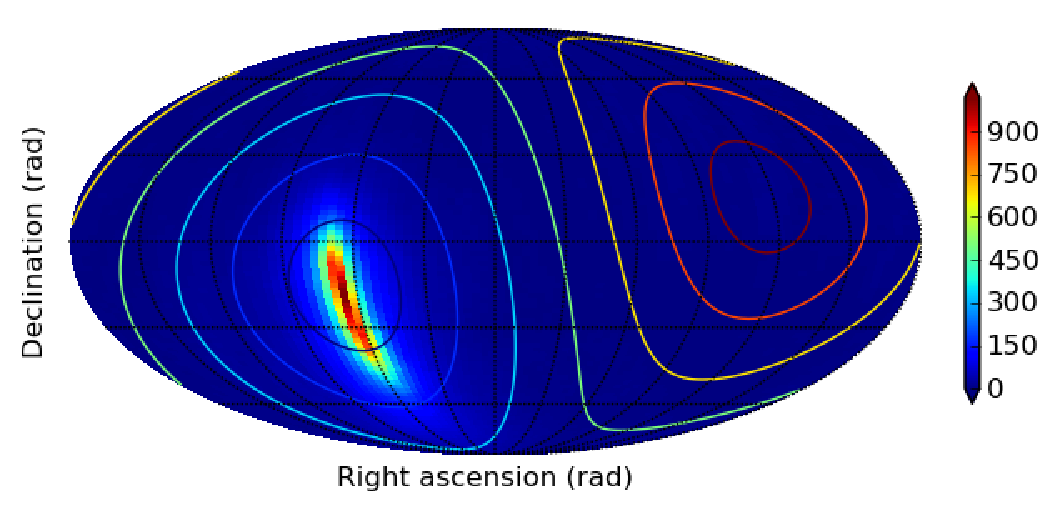
\includegraphics[width=0.4\paperwidth,height=0.2\paperheight]{maptrueH1}}
%\protect\caption{\protect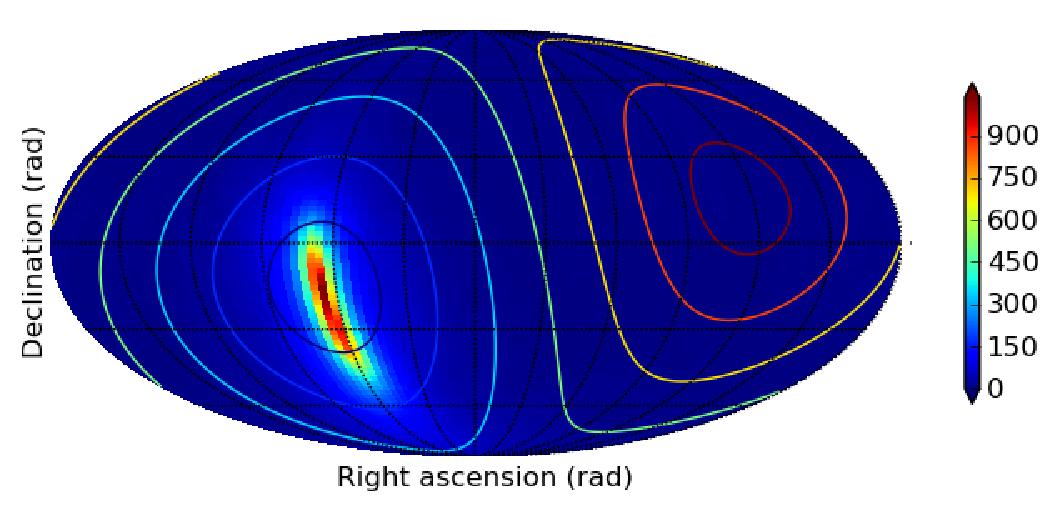
\includegraphics[width=0.4\paperwidth,height=0.2\paperheight]{maptrueL1}}
%\protect\caption{\protect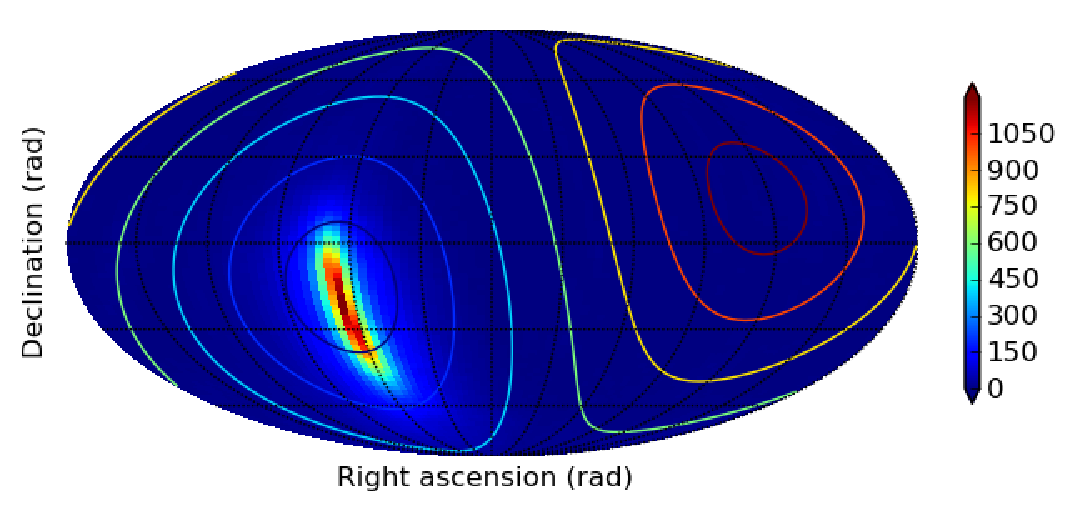
\includegraphics[width=0.4\paperwidth,height=0.2\paperheight]{maptrueV1}}
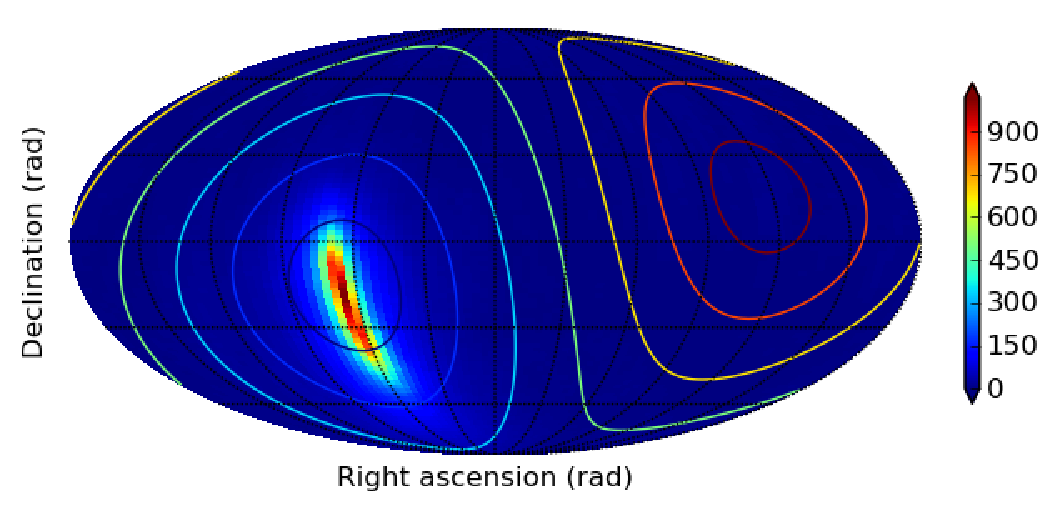
\includegraphics[width=0.6\paperwidth,height=0.2\paperheight]{maptrueH1.eps}
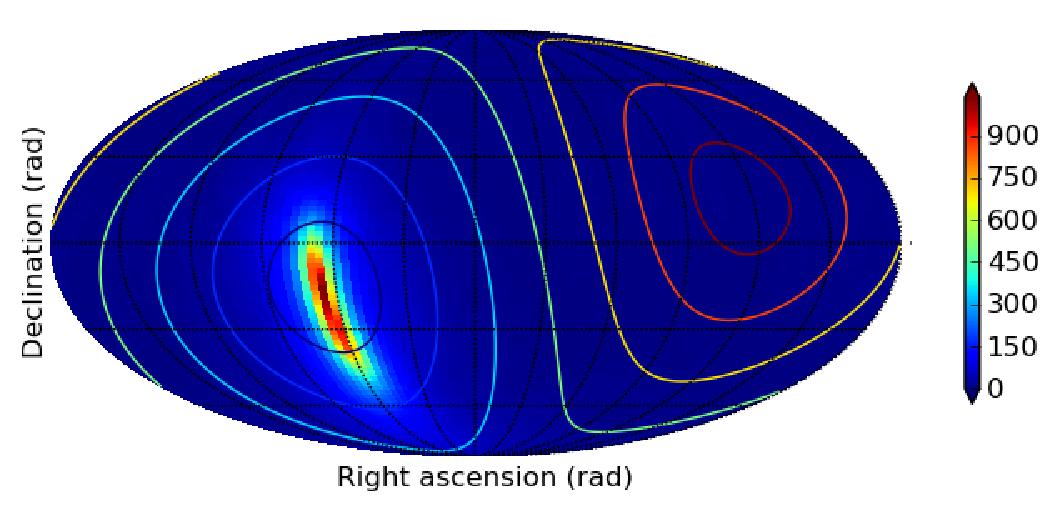
\includegraphics[width=0.6\paperwidth,height=0.2\paperheight]{maptrueL1.eps}
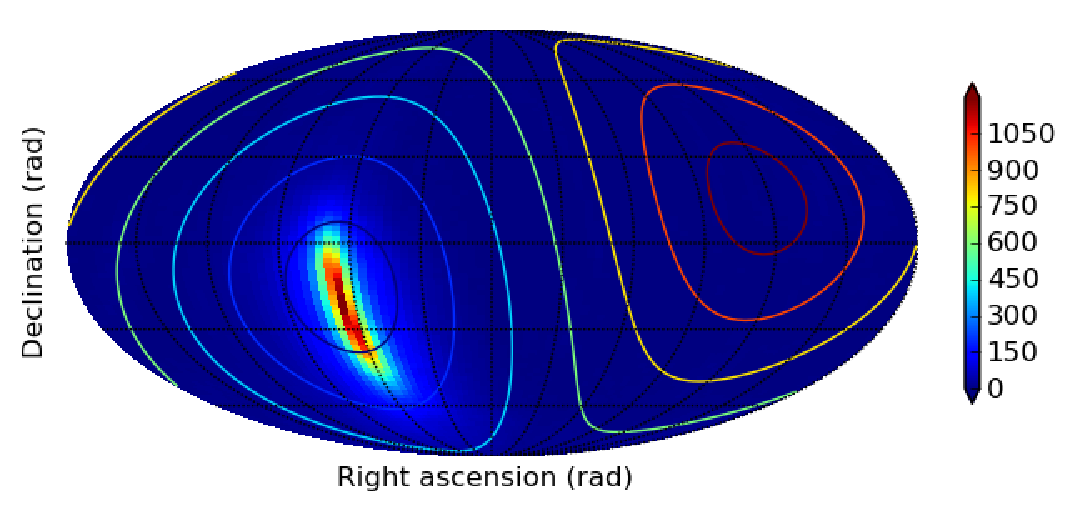
\includegraphics[width=0.6\paperwidth,height=0.2\paperheight]{maptrueV1.eps}
\caption{ All-sky maps, \{H1, L1, V1\} interferometer analysis from top to bottom, for template tests varying right ascension and declination. 
Scorpius X-1 mock data challenge pulsar 16 (101x101 templates), showing $\log_{10}p$-value on a Mollweide projection.
Contour lines at 1-radian great-circle distance intervals from the intended injection location of Sco X-1.
The results match the intended injection and confirm that the simulation is accurately representing the known sky location of Sco X-1.
}
\label{scox1-allsky-maps}
\end{center}
\end{figure}

At the beginning of the MDC, this author's work on TwoSpect played a key role in verifying that the simulation was correctly set up.
Although the author played no role in the data generation -- and was blinded to the parameters of the closed pulsars -- TwoSpect is sensitive both to relatively-weak signals and to sky location.
Thus it was able to confirm that injected pulsars, as seen in Figure~\ref{scox1-allsky-maps}, were in fact in the expected location of a signal from Scorpius X-1.

%\end{frame}

\section{Scorpius X-1 mock data challenge}
%\begin{frame}{Fully-templated search for Scorpius X-1}
\subsection{Fully-templated search for Scorpius X-1}


\begin{figure}
\begin{center}
%\protect\caption{\protect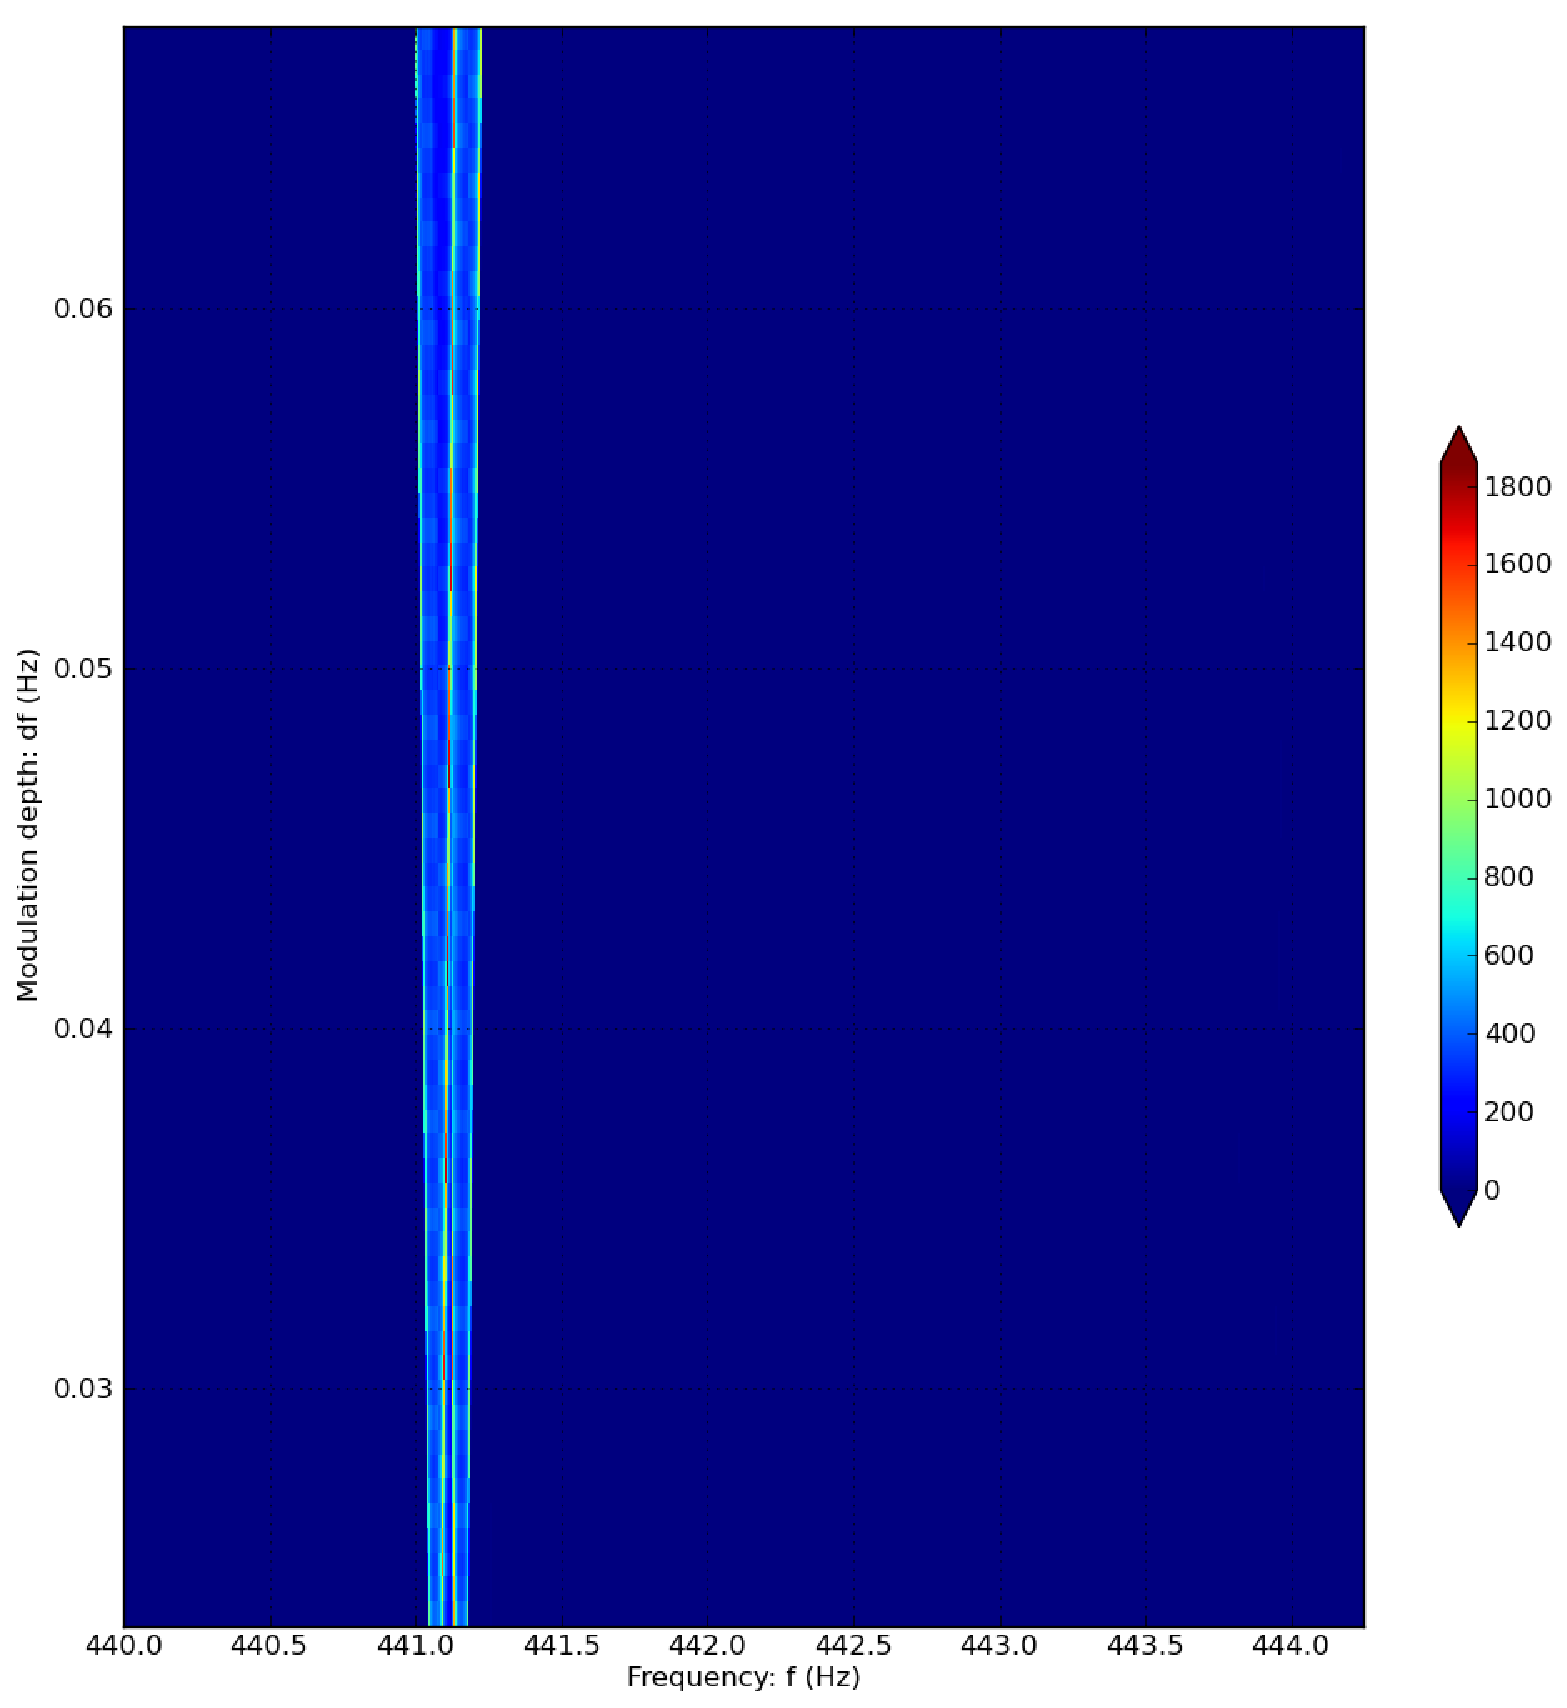
\includegraphics[width=0.8\paperwidth,height=0.62\paperheight]{bandH1-bold}}
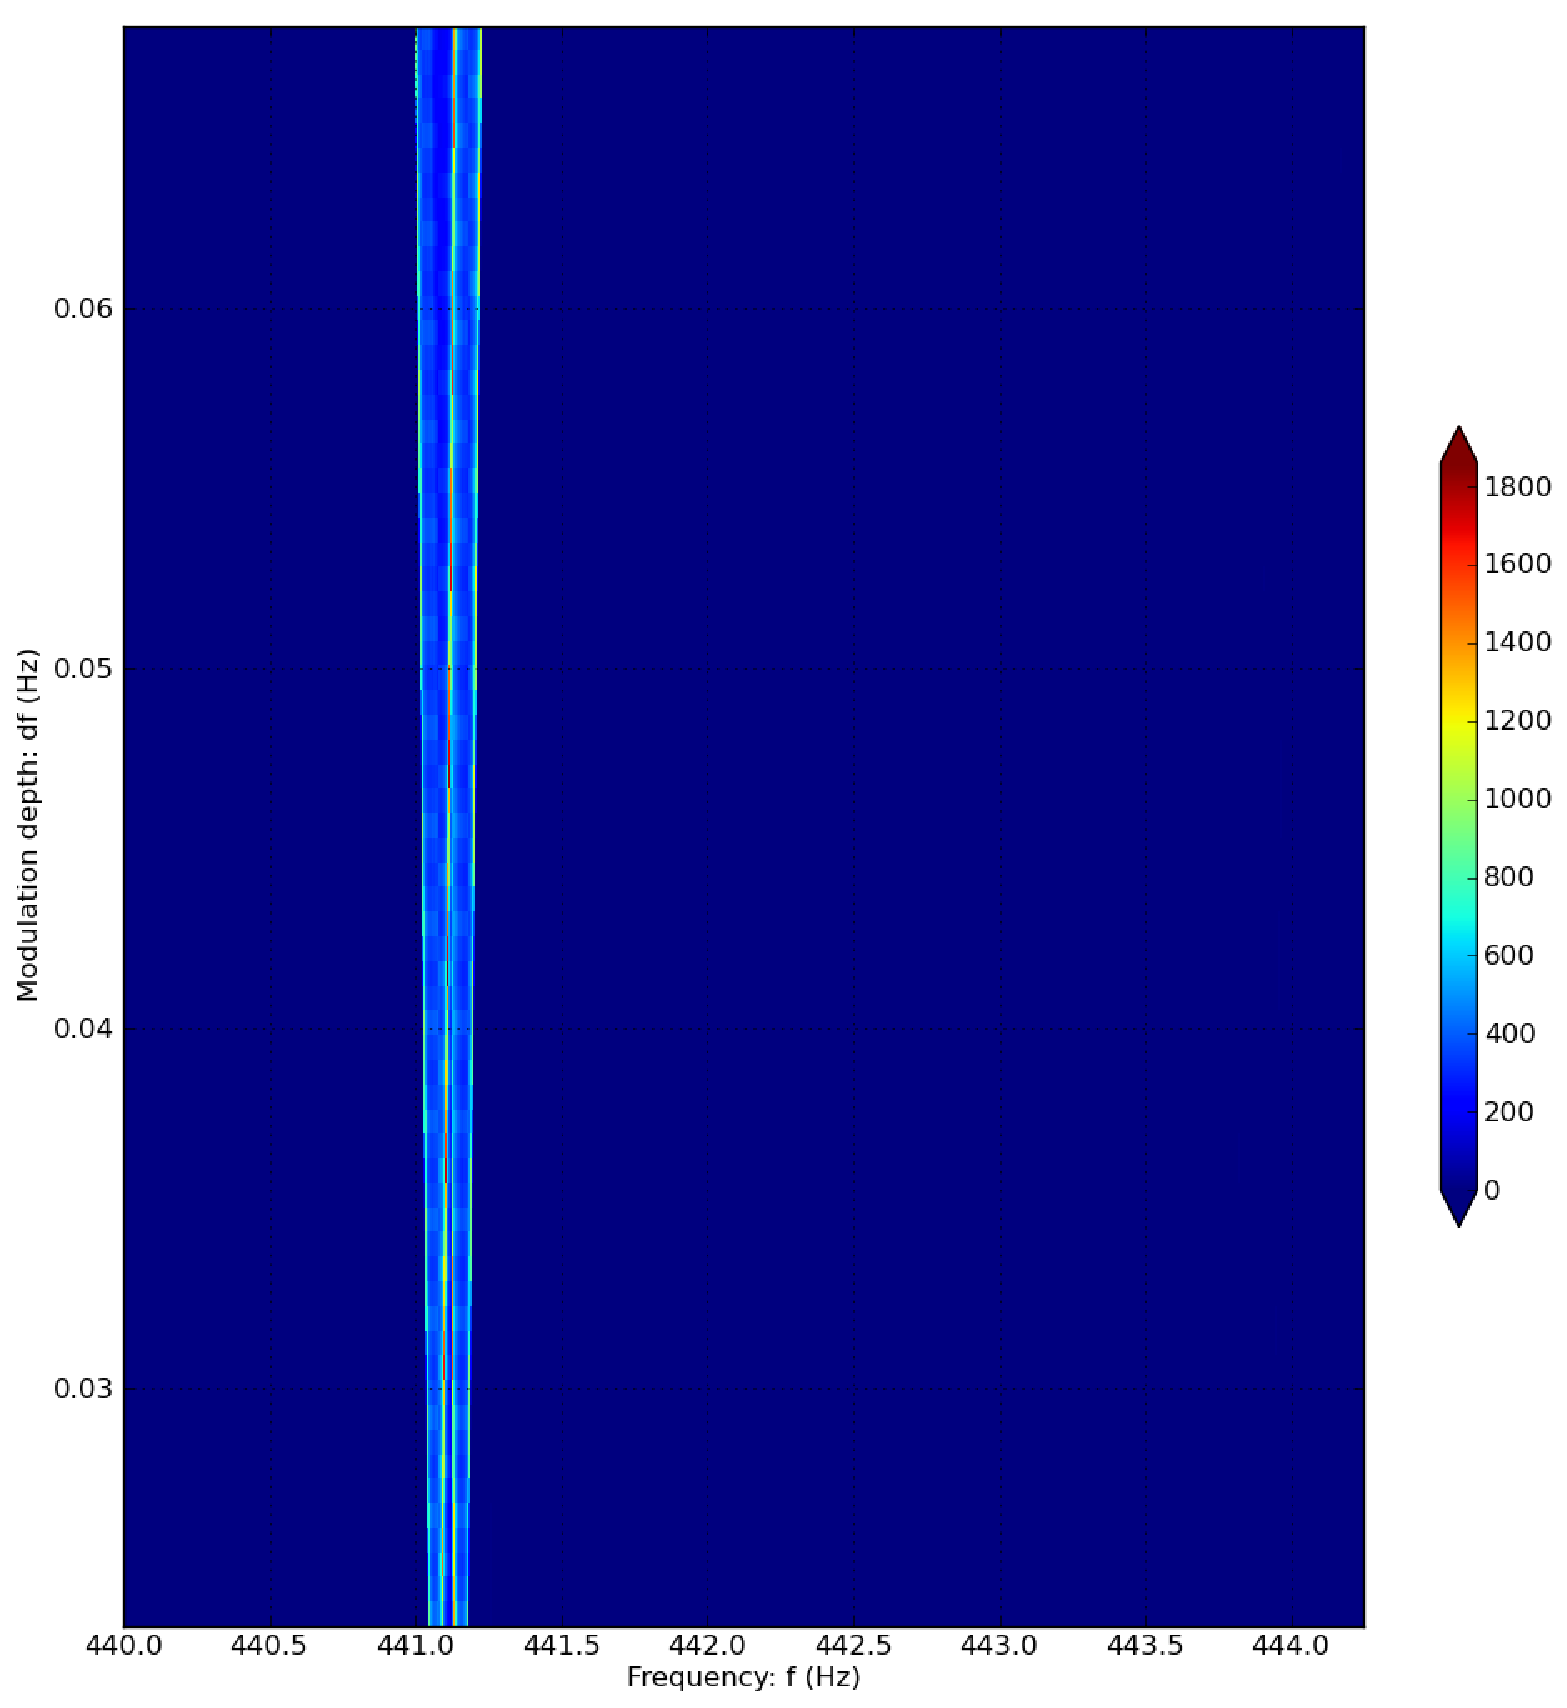
\includegraphics[width=0.8\paperwidth,height=0.62\paperheight]{bandH1-bold.eps}
\caption{
Scorpius X-1 Mock Data Challenge (MDC) pulsar 40 \{H1\}: 5 Hz band. 
The $p$-value (single-template, applying Davies' Method to the $R$ statistic) in is show in this heatmap, peak in red. 
All templates are plotted on the (frequency, modulation depth) plane.
This is a relatively broadband view.
}
\label{scox1-wide-heatmap-040}
\end{center}
\end{figure}

Scorpius X-1 MDC data necessitated a efficient means of searching over a few hundred million putative templates using similar data streams from three interferometers (Hanford H1, Livingston L1, and Virgo V1).
Ideally, all one hundred 5 Hz search bands would be illuminated in the manner of Figure~\ref{scox1-wide-heatmap-040}.
Achieving this goal required some development by the author.

%\end{frame}

%\begin{frame}{Narrow-band heat maps in parameter space}
\subsection{Narrow-band heat maps in parameter space}


\begin{figure}
\begin{center}
%\protect\caption{\protect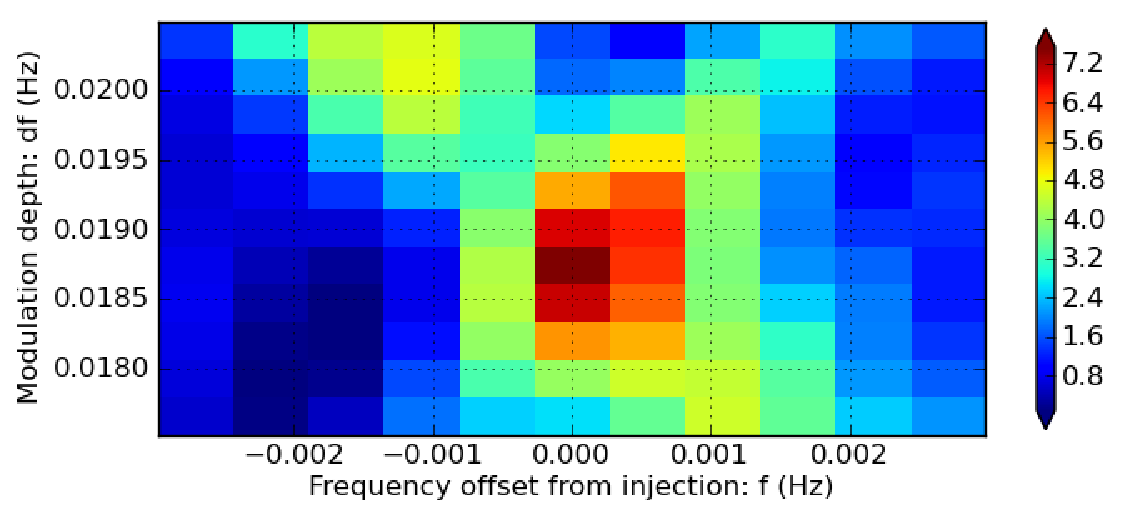
\includegraphics[width=0.4\paperwidth,height=0.2\paperheight]{heatmapH1}}
%\protect\caption{\protect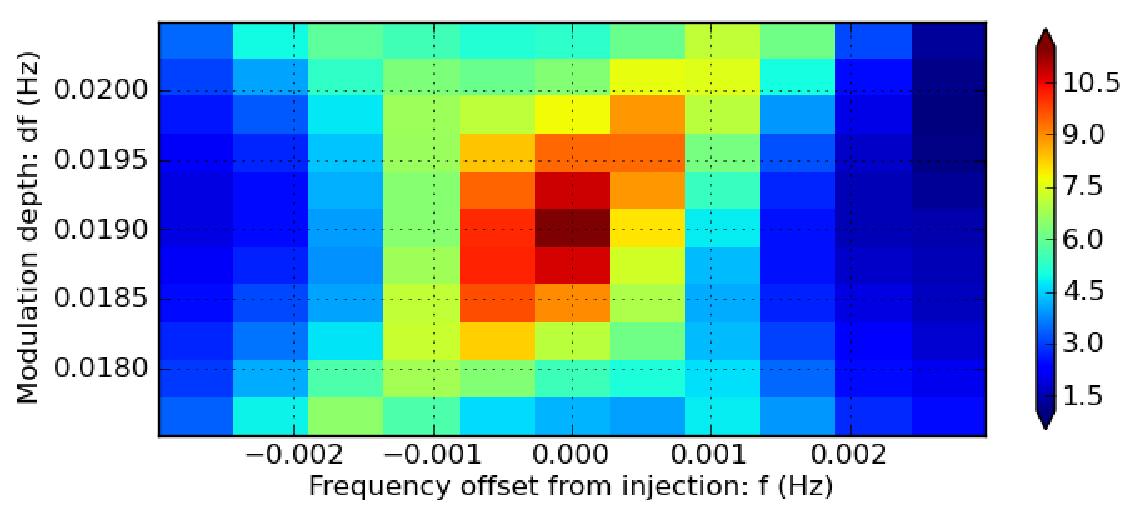
\includegraphics[width=0.4\paperwidth,height=0.2\paperheight]{heatmapL1}}
%\protect\caption{\protect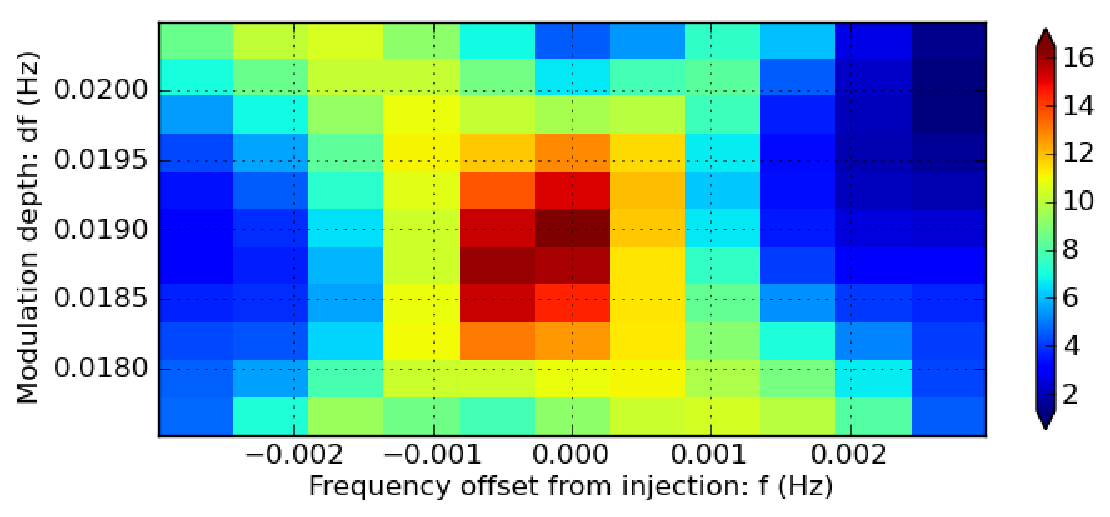
\includegraphics[width=0.4\paperwidth,height=0.2\paperheight]{heatmapV1}}
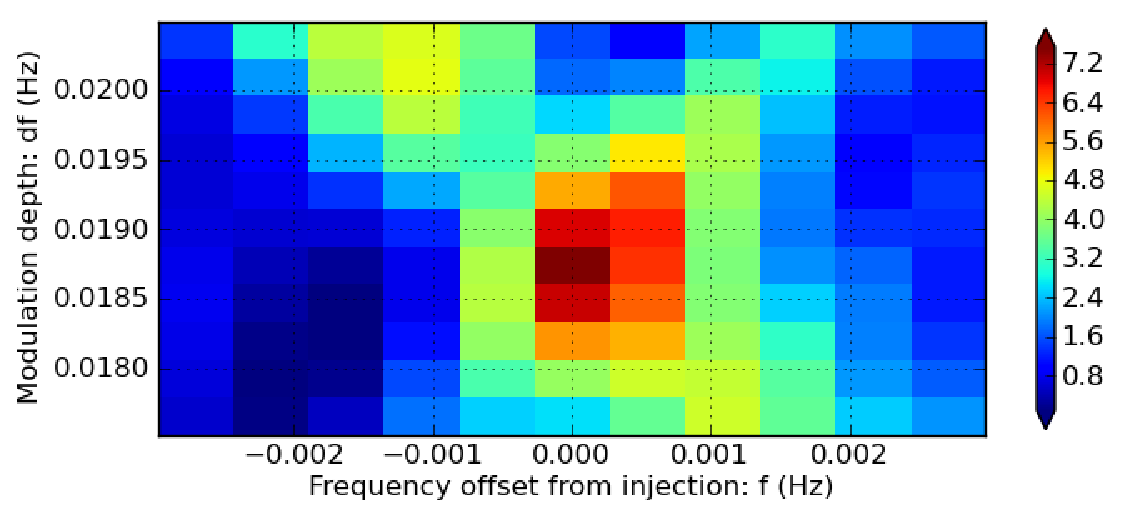
\includegraphics[width=0.6\paperwidth,height=0.2\paperheight]{heatmapH1.eps}
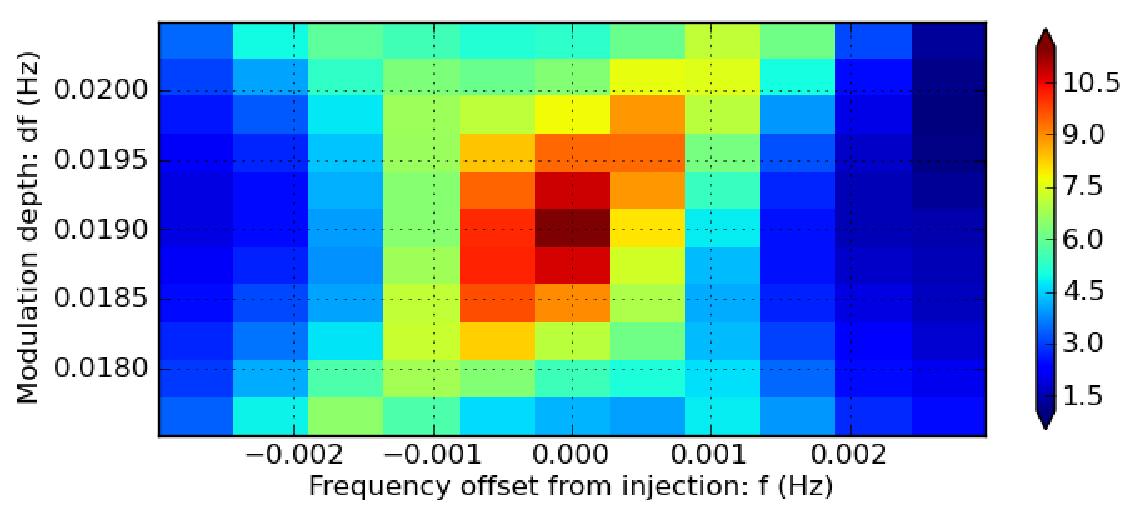
\includegraphics[width=0.6\paperwidth,height=0.2\paperheight]{heatmapL1.eps}
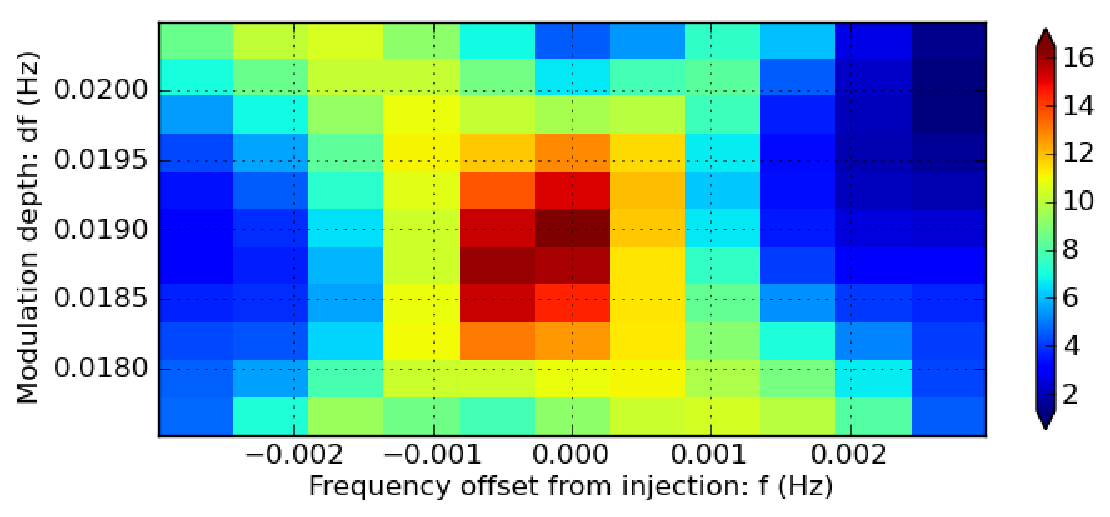
\includegraphics[width=0.6\paperwidth,height=0.2\paperheight]{heatmapV1.eps}
\caption{Heatmaps \{H1, L1, V1\} of 11x11 templates centered around
Scorpius X-1 MDC pulsar 8. 
This is a relatively narrowband view.
}
\label{scox1-narrow-heatmap-008}
\end{center}
\end{figure}

Initially, TwoSpect was configured for all-sky searches with the capability to bypass the incoherent harmonic sum and test a single point in parameter space.
It was possible to test multiple templates only by rerunning the entire TwoSpect pipeline.
Initial input/output loaded and Doppler-shifting made this highly-wasteful, although it was possible to obtain results in narrow regions around which the unblinded, open MDC pulsars were specified.
Figure~\ref{scox1-narrow-heatmap-008} illustrates one such result.

%\end{frame}

%\begin{frame}{Wide-band heat maps in parameter space}
\subsection{Wide-band heat maps in parameter space}

\begin{figure}
\begin{center}
%\protect\caption{\protect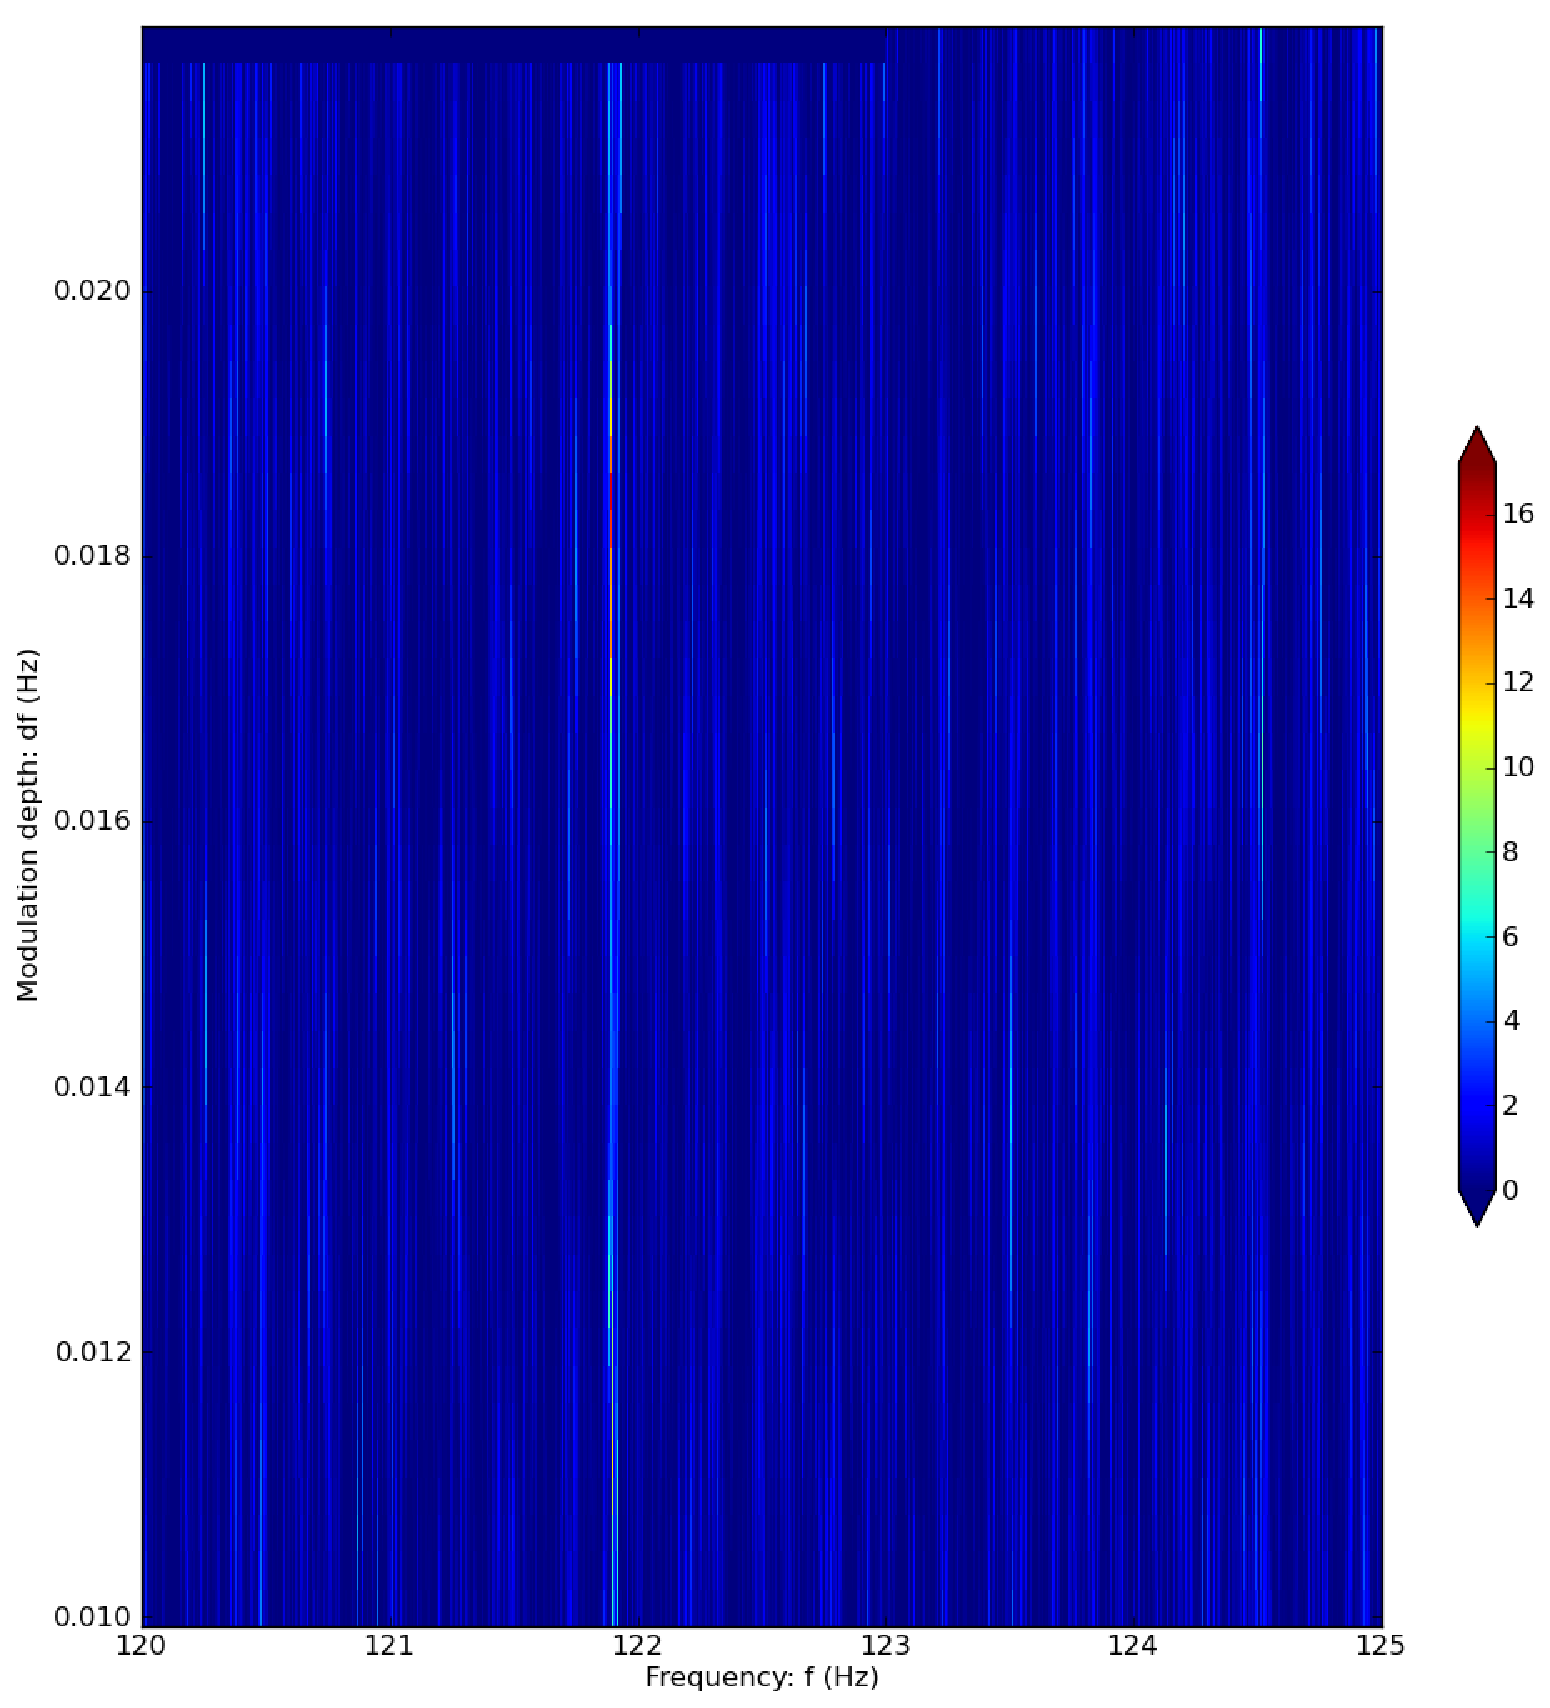
\includegraphics[width=0.8\paperwidth,height=0.62\paperheight]{bandH1}}
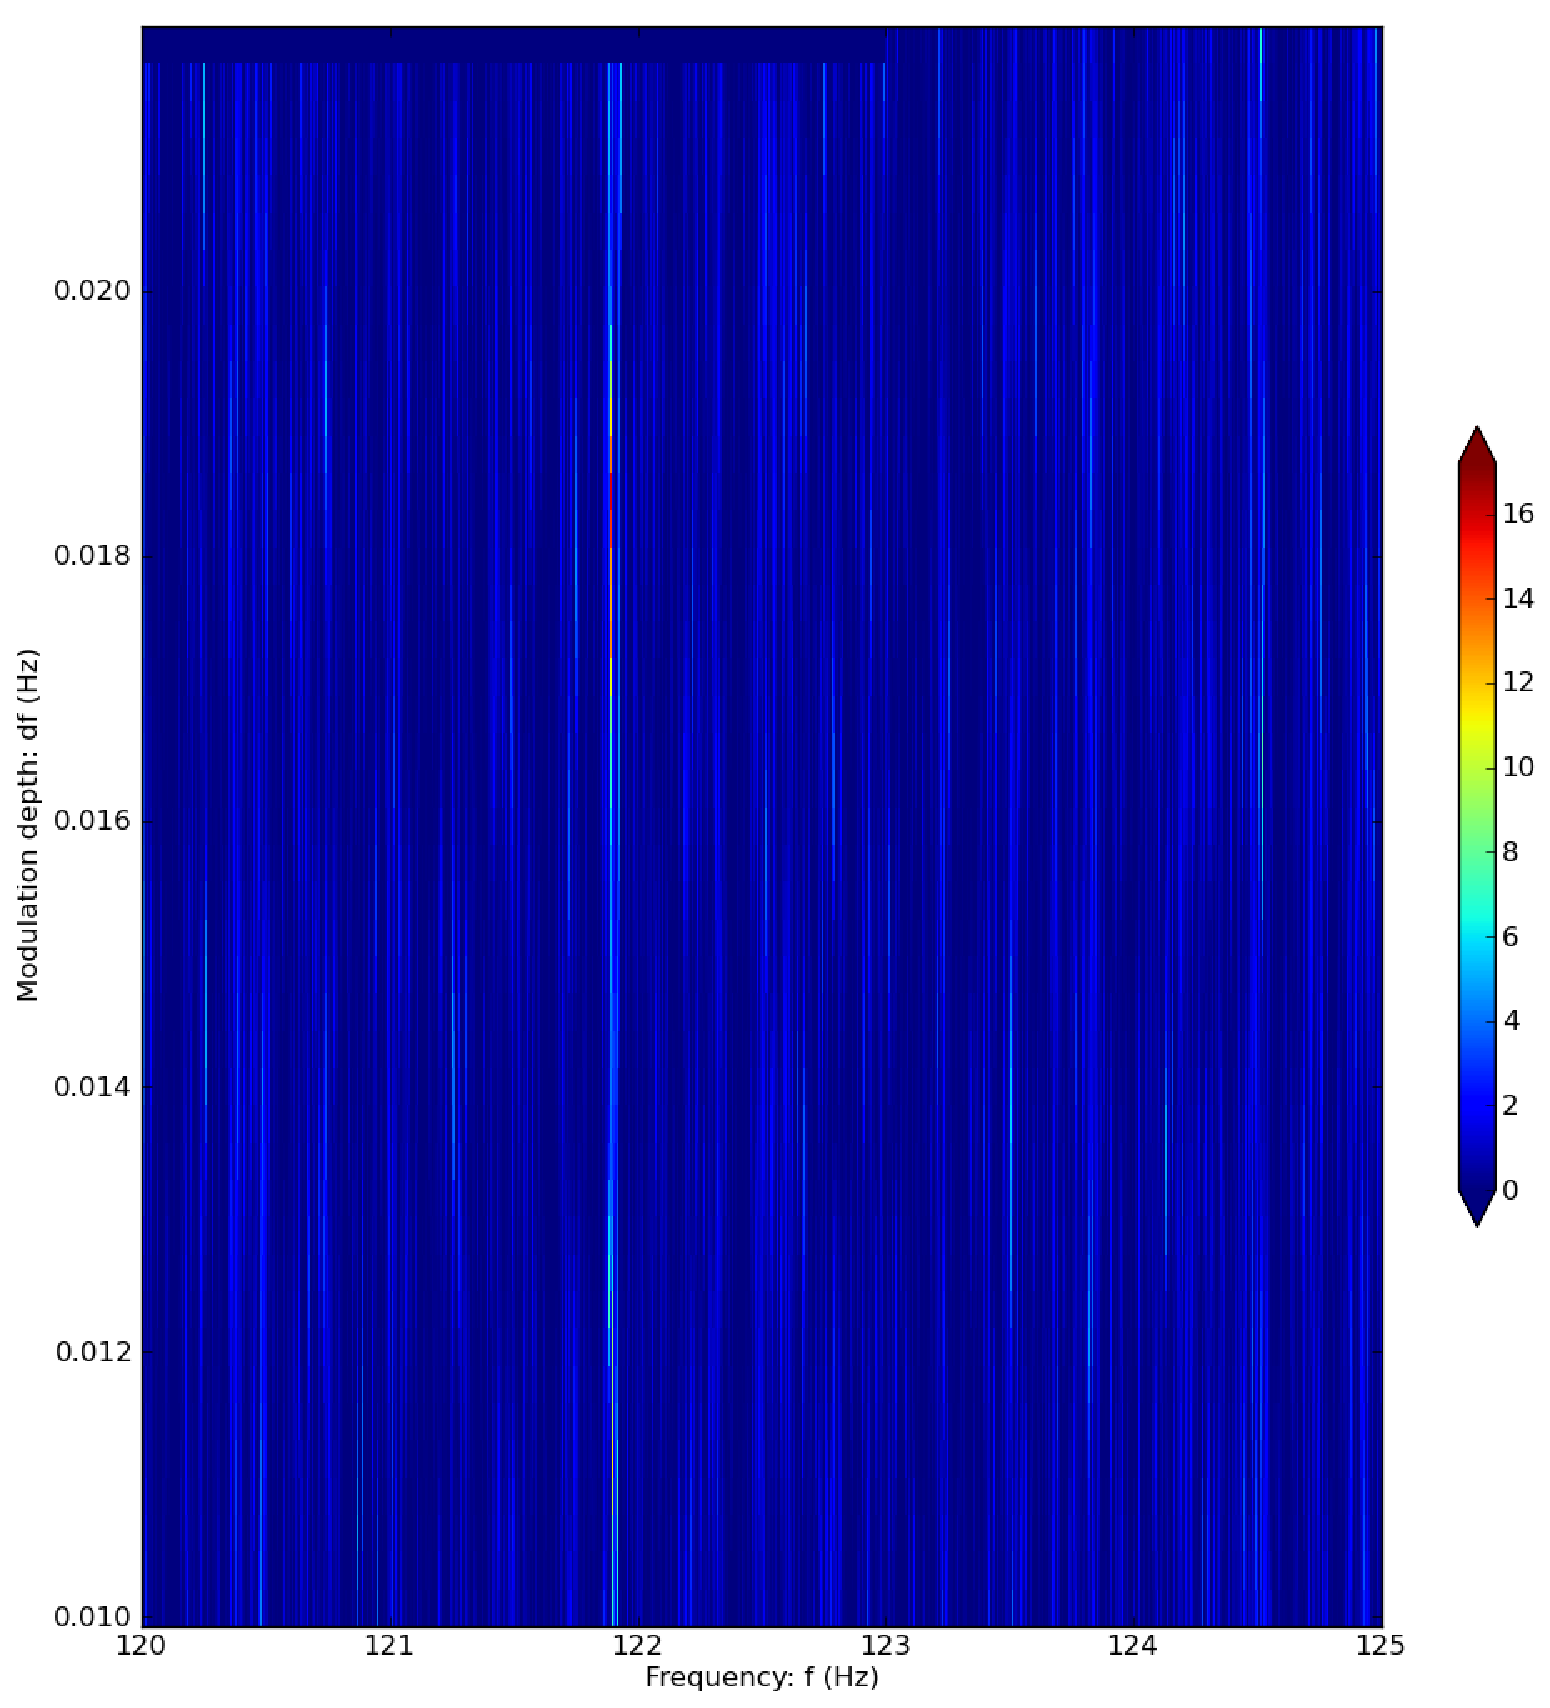
\includegraphics[width=0.8\paperwidth,height=0.62\paperheight]{bandH1.eps}
\caption{Scorpius X-1 MDC pulsar 8 \{H1\}: 5 Hz band. This heatmap shows $3.6\times10^{5}$ templates, 10 to 22 mHz modulation depth, 120-125 Hz frequency. The peak signal at about (df = 0.019, f = 121.9) Hz.
}
\label{scox1-wide-heatmap-008}
\end{center}
\end{figure}

The author's first contribution to the pipeline was by streamlining searching over arbitrary-width frequency bands.
Input/output is now done only once for a given search band, as is Doppler-shifting, expediting the testing of many templates for the $R$-statistic by several orders of magnitude.
While testing so many templates is arguably unnecessary -- the results are highly correlated -- it is computationally straightforward and yields the best gain in sensitivity over previous searches.
Figure~\ref{scox1-wide-heatmap-008} shows that these results match up with prior work, from Figure~\ref{scox1-narrow-heatmap-008}.

Whereas much existing TwoSpect post-processing to data had been focused on follow-up of all-sky results, parts of the directed search post-processing have needed to be re-invented.
The MDC validated these methods.

%\end{frame}

%\begin{frame}{Revisiting \& refining detection criteria}
\subsection{Revisiting \& refining detection criteria}


\begin{figure}
\begin{center}
%\protect\caption{\protect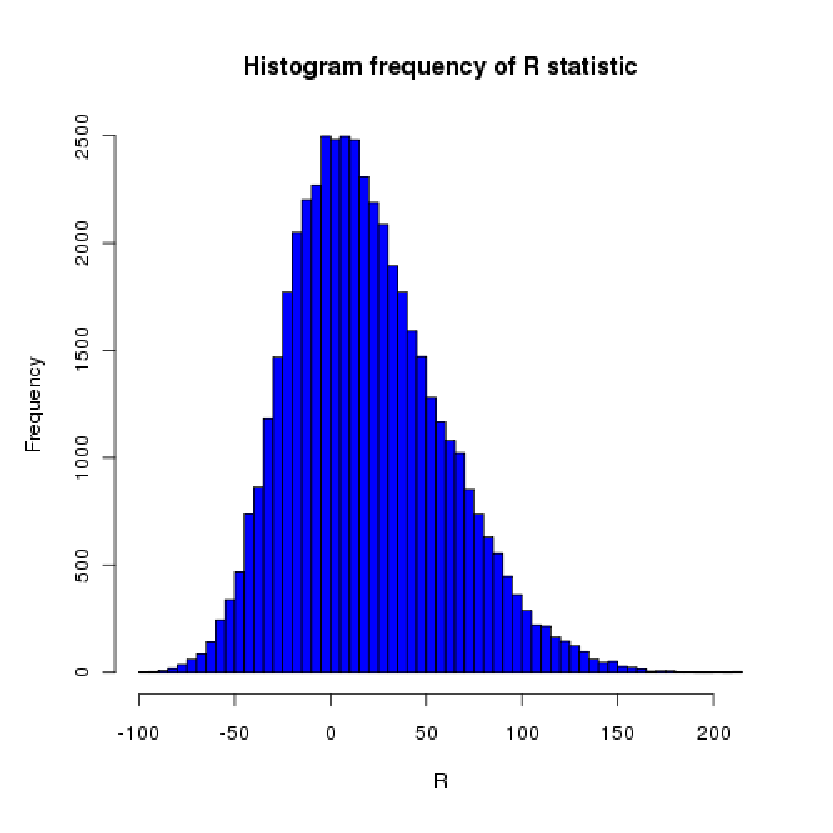
\includegraphics[width=0.45\paperwidth,height=0.45\paperheight]{StatHistRH1}\protect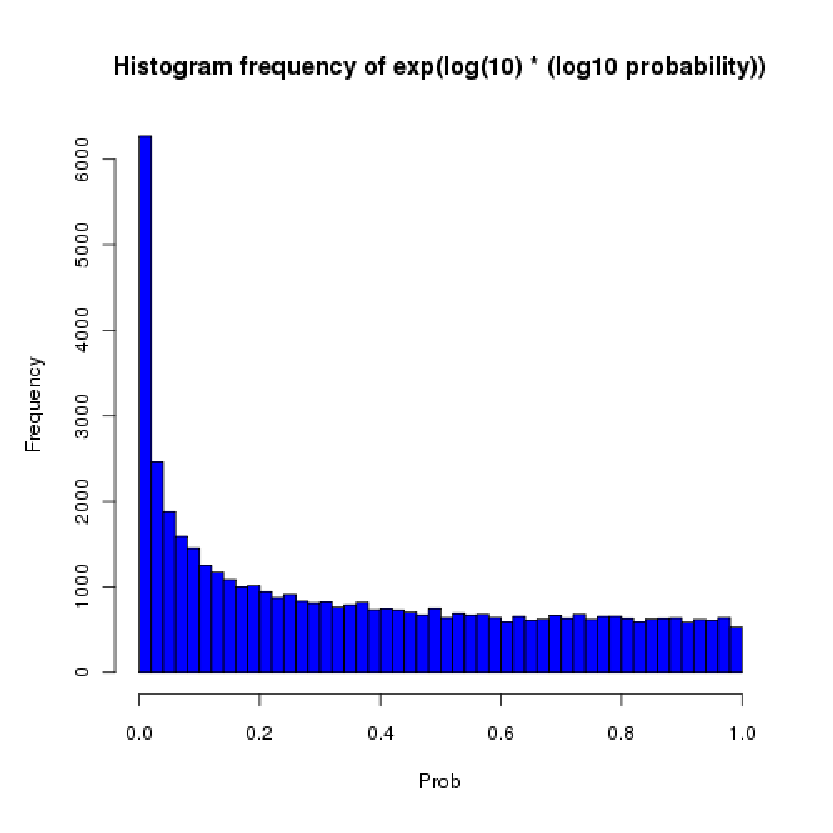
\includegraphics[width=0.45\paperwidth,height=0.45\paperheight]{StatHistProbH1}}
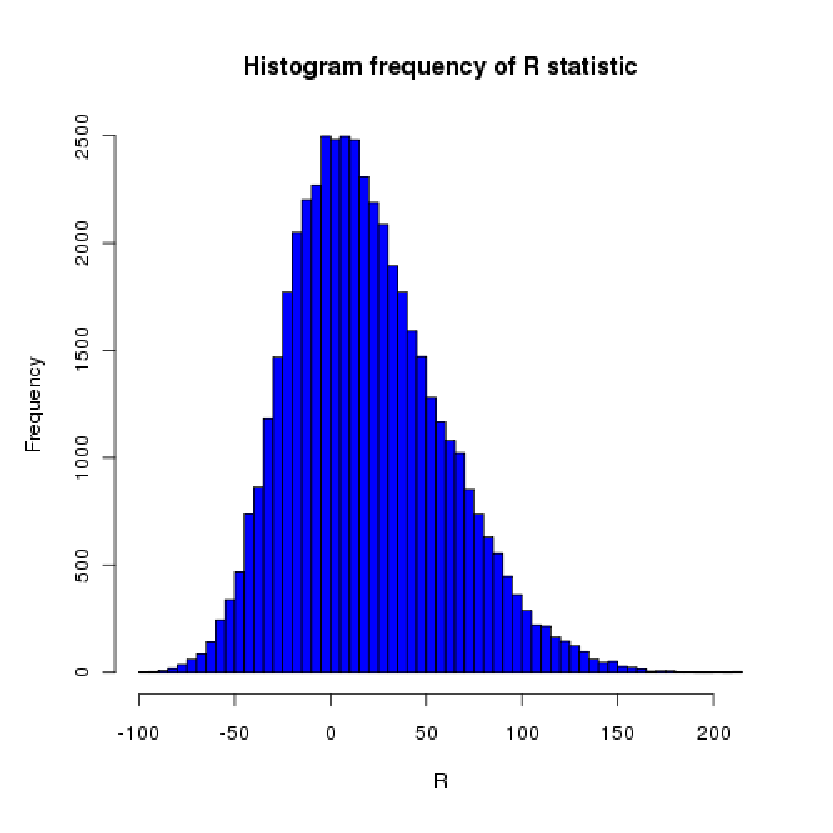
\includegraphics[width=0.6\paperwidth,height=0.35\paperheight]{StatHistRH1.eps}
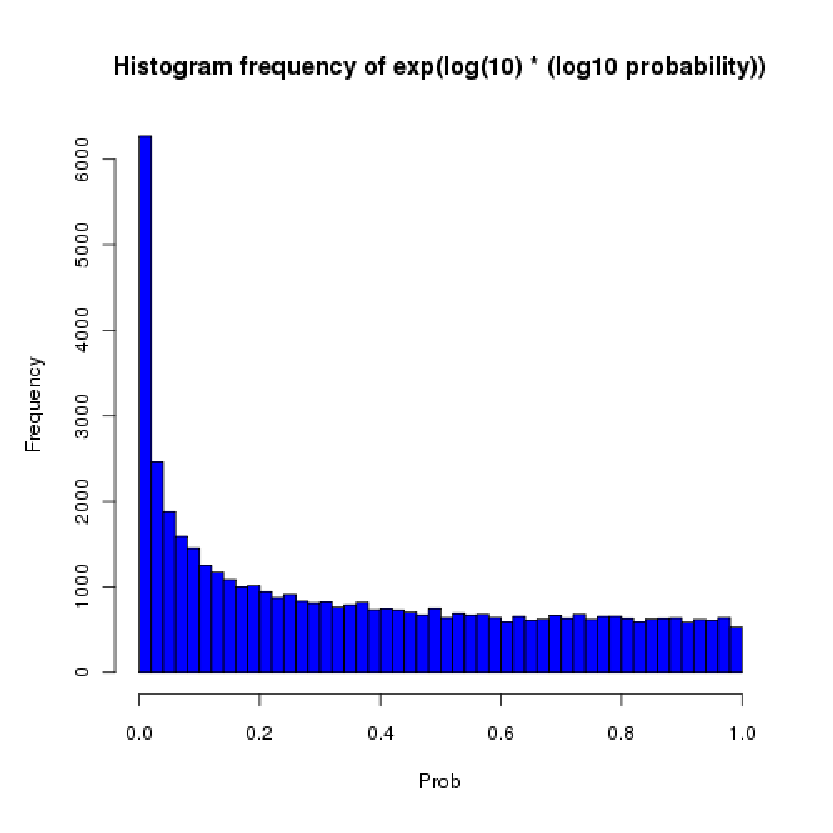
\includegraphics[width=0.6\paperwidth,height=0.35\paperheight]{StatHistProbH1.eps}
\caption{Scorpius X-1 MDC statistics. These histograms of the $R$ statistic and $p$-value distribution were part of understanding noise, temporal gap \& spectral leakage, as well as establishing a threshold $p$-value $\sim$ false alarm probability of 1\%.
These $p$-values are for single templates, appropriate to the all-sky search but not to a dense templated search with a large trials factor.
Here, histograms show statistics in the absence of a signal. 
The left-skew of the $p$-values is associated with gaps in the data (as is right-skew, with different gaps).
Diurnal bias in barycentering is assumed, but the correlation is not fully understood.
}
\end{center}
\end{figure}



Running TwoSpect as a directed search algorithm involves calculating
the $R$-detection statistic across the probable parameter space. 
A search is conducted with templates for each grid point in the Scorpius 
X-1 parameter space; period is known sufficient well to restrict the search
to the two dimensions of signal frequency and frequency modulation. The
grid spacing, inversely proportional to spectrum coherence time, was
chosen to allow a mismatch no more than $0.2$ in the detection statistic.
Due to known period and sky location, the incoherent harmonic sum stage
of TwoSpect, used for the all-sky search, was bypassed entirely. 

\section{Mock Data Challenge procedure}

Each interferometer in the data challenge was analyzed individually for 
the detection statistic and corresponding single-template $p$-value. A set
of highest $p$-value outliers in 5 Hz bands were produced for each 
interferometer, subject to a $p$-value threshold inferred from Gaussian noise.
These sets were compared in pairwise coincidence (H1-L1, H1-V1, or L1-V1),
where coincidence required proximity within a few grid points in the 
parameter space. Any surviving outliers were classified as a detection. 

The highest $p$-value outlier in a single interferometer in that band 
yielded the estimated parameters. Uncertainties in these parameters were also
determined from unblinded injections, using method of moments for signal
frequency and modulation depth and confidence intervals for signal
amplitude. Upper limits were declared from the best estimate of the 95
percent confidence level of non-detected unblinded injected signals. The
largest uncertainty in upper limits and signal amplitude estimation derives
from the ambiguity in between true $h_0$ signal and $\cos \iota$ inclination.
This ambiguity cannot be resolved with the present algorithm and depends
partially on the assumed prior distribution of signal ampltitudes; the
uncertainty was estimated by simulation.

Put another way, TwoSpect
in its directed search mode, tests templates with a model of
$f$, $a \sin i$, and $P$, as well as sky location. The latter two are
fixed for Scorpius X-1 are they are well-known. 
It is not sensitive to time of ascension.
If a coincident detection is made between any interferometer pair in a 5 Hz band,
model parameters are read off from the extremal $p$-value template at
any one interferometer; $h_0$ is proportional to the quarter-root of
the test statistic. Uncertainty in $f$ and $a \sin i$ is determined
from the standard deviation of known injections; it is on the scale
of the template grid except for marginally-detected pulsars. The $h_0$ 
uncertainty is largely due to the distribution of $\cos \iota$. 

TwoSpect claimed to detect 34 of 50 blinded signals, as well as 31 of 50 unblinded signals, and it stated a flat
$4.23 \times 10^{-25}$ upper limit for the 16 non-detected signals. 

\subsection{Detection Claims}

After studying the Gaussian noise in the Scorpius X-1 MDC open data set, we were able to set thresholds for detection claims.

TwoSpect's $R$-statistic and $p$-value space on {frequency}x{modulation depth} showed significant structures, particular around loud injections, corresponding to the distribution of power into pixels by way of modulation depth, Earth's Doppler motion, and possibly spectral leakage. These regions of the open data set parameter space were excised before proceeding with the Gaussian noise study.

TwoSpect also found differences in the noise between the 360 s SFTs, used for pulsar bands above 360 Hz, and the 840 s SFTs, used for those bands below. The shorter SFTs were noisier.

After studying the effect of pairwise coincidence requirements on surviving Gaussian noise outliers, we were satisfied that we would achieve a false alarm rate of 0.01 or better by setting the following detection criteria. Note that the $\log_{10} p$ values refer to single-template $p$-values, which are generally correlated with each other.

\subsection{Detection criteria}

\begin{itemize}
\item each candidate must survive at least one double-IFO coincidence test, involving a pairwise comparison of single-IFO candidates to see whether they are within 1/$T_{\textup{SFT}}$ in both frequency ($f$) and modulation depth ($df$).
\item single-IFO candidates are the up-to-200 most extreme $p$-value outliers in a 5 Hz band that had a $\log_{10}p \leq$ threshold, where threshold = -7.75 if $f <$ 360.0 Hz (those that used 840 s SFTs) or -12.0 if $f \geq$ 360.0 Hz (those that used 360 s SFTs).
\end{itemize}

$\rightarrow$ if there is any candidate surviving these criteria in a 5 Hz band, we mark detected, else not detected

\subsection{Parameter Estimation}

Open MDC data gave TwoSpect the the ability to check its parameter estimation on the 31 pulsars detected in the open data set.

Note that the $h_0$ reported in this section had not yet been recalibrated for either the $\cos \iota$ ambiguity due to assumed circular polarization (see subsequent section, factor of 1.74) or a systematic rescaling endemic to TwoSpect (factor of 1.11). Instead, the first step was to rescale the known $h_0$-injected from the MDC open data table into an h-effective. This h-effective equaled $\sqrt{ ((1+\cos^2 \iota) / 2)^2 + (\cos \iota)^2 }/\sqrt{2}$ * $h_0$-injected, the rescaling necessary to convert the strain into effective units of circular polarization strain. Any pipeline that assumes circular polarization should require a similar procedure.

We plotted the error in the $h_0$ reported by TwoSpect versus $h_0$-effective for the 31 open pulsars detected.


\begin{figure}
\begin{center}
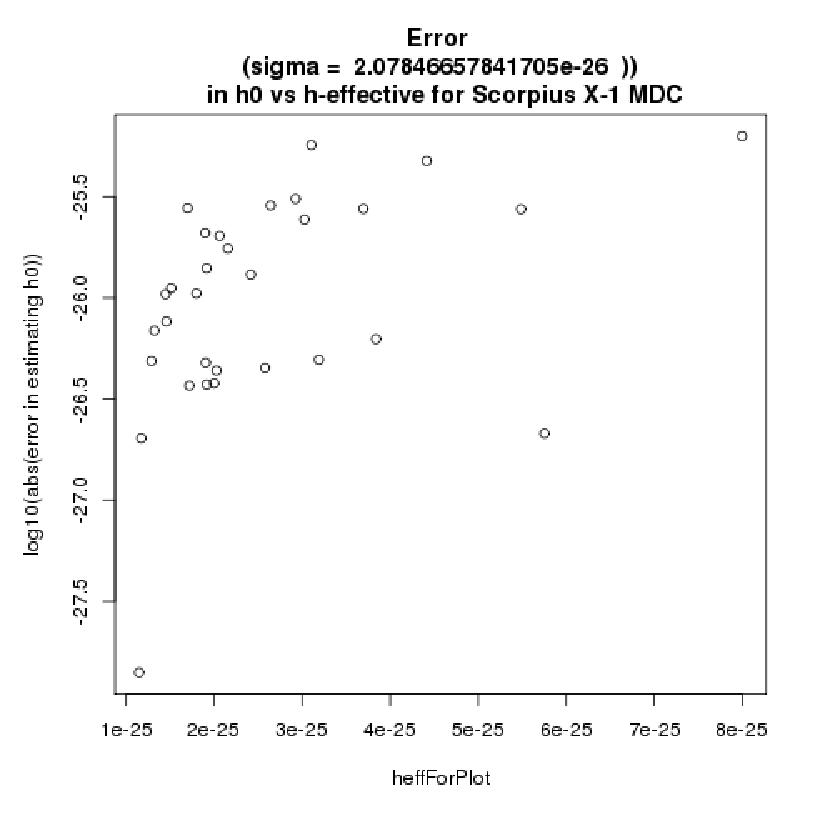
\includegraphics[width=0.3\paperwidth,height=0.2\paperheight]{detectedHerrVsHeffective.eps}
\caption{ Error in strain estimation versus circular-effective injected strain. Higher injected strain results in higher absolute errors.
\label{fig:detectedherrvsheffective}} 
\end{center}
\end{figure}


This same error was also plotted vs $p$-value and frequency, Figure~\ref{fig:errorh0}. As will be seen on the plots for error in frequency and asini, high-frequency outliers were found in the open data set. These outliers could be categorized heuristically as having $f >$ 1050 Hz and abs($\log_{10}p$) $<$ 300. These 4 outliers were assigned into the \textit{loose} category, with a corresponding $\sigma$. The remaining 27 were in the \textit{tight} category, to which we could assign a more stringent $\sigma$. Later, it was found that the high-frequency outlier behavior could mostly be explained by a misconfiguration bug where TwoSpect was not asked to retrieve needed SFT data; the rerun plots show a lower \textit{overall} uncertainty. These values are reported in the header of the graphs.

Blue lines indicate the less stringent uncertainty. Red lines (on plots vs $p$-value) indicate a least squares power law regression.

\begin{figure}
\begin{center}
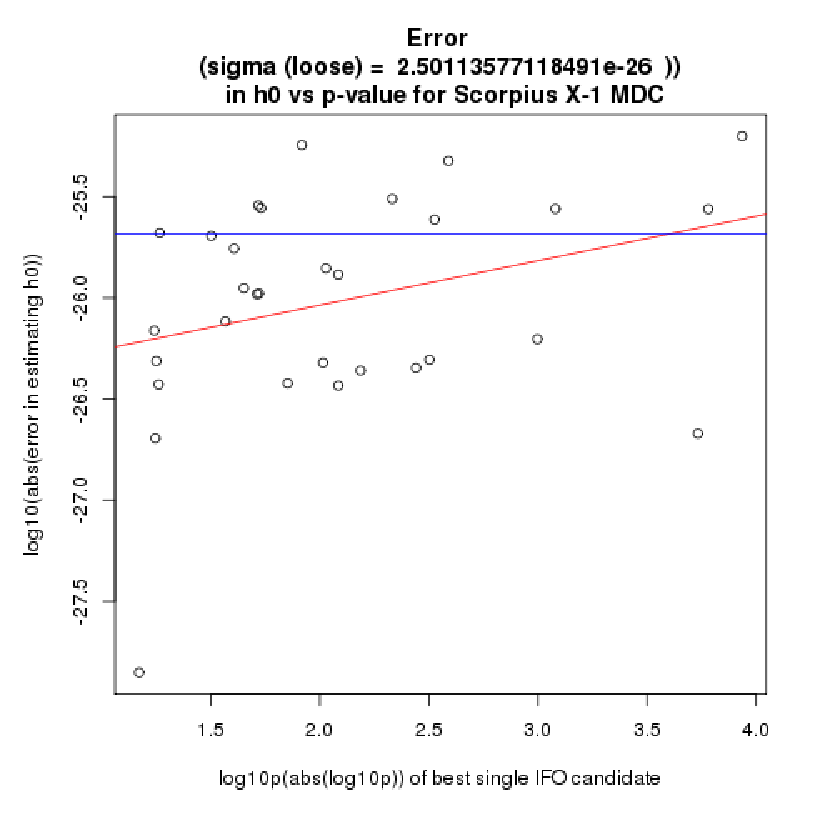
\includegraphics[width=0.3\paperwidth,height=0.2\paperheight]{Errorh0.eps}
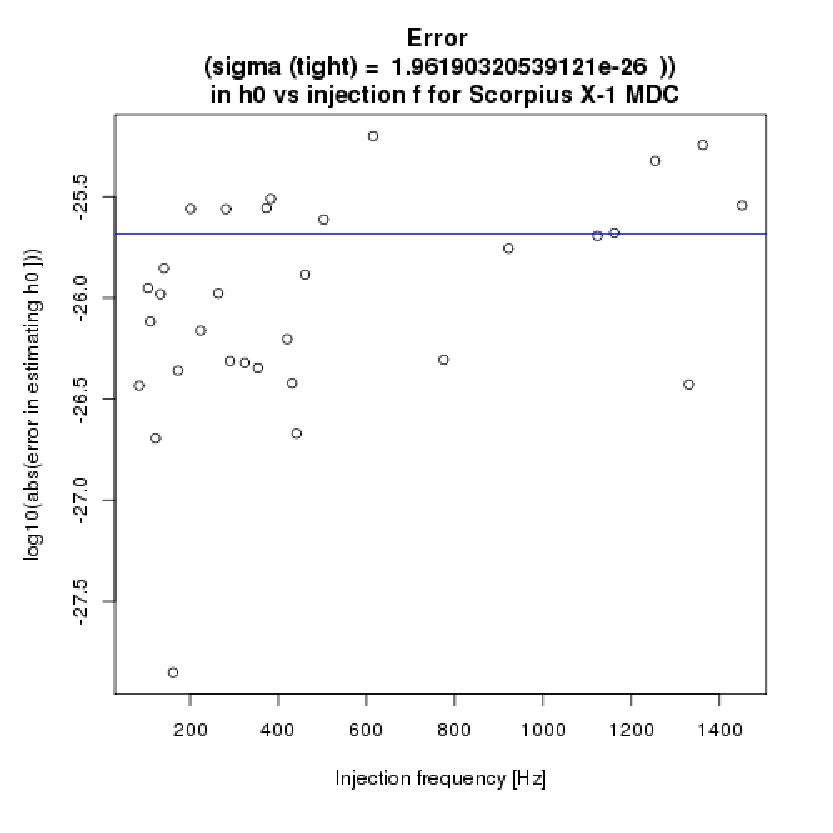
\includegraphics[width=0.3\paperwidth,height=0.2\paperheight]{Errorh0vsF.eps}
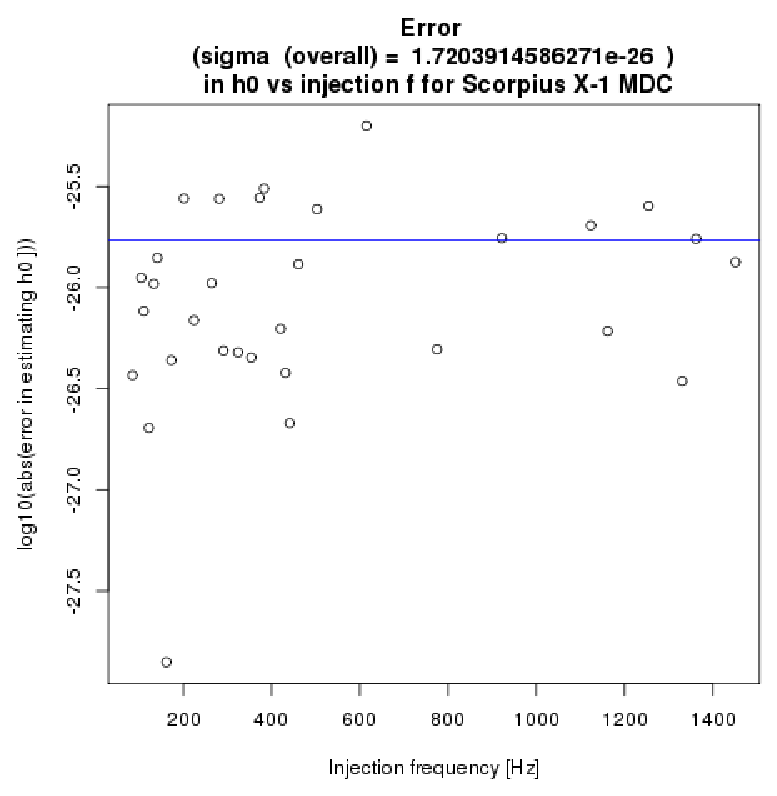
\includegraphics[width=0.6\paperwidth,height=0.4\paperheight]{plots/Errorh0vsF-overall.eps}
\caption{Parameter estimation: error in strain as a function of recovered $p$-value (top left) and frequency (top right). The strain appears broadly distriuted, without any systematic patterns. The overall error vs frequency is shown at bottom after a rerun to fix a misconfiguration where inadequate data was read-in at high frequencies.
\label{fig:errorh0}}
\end{center}
\end{figure}


\begin{figure}
\begin{center}
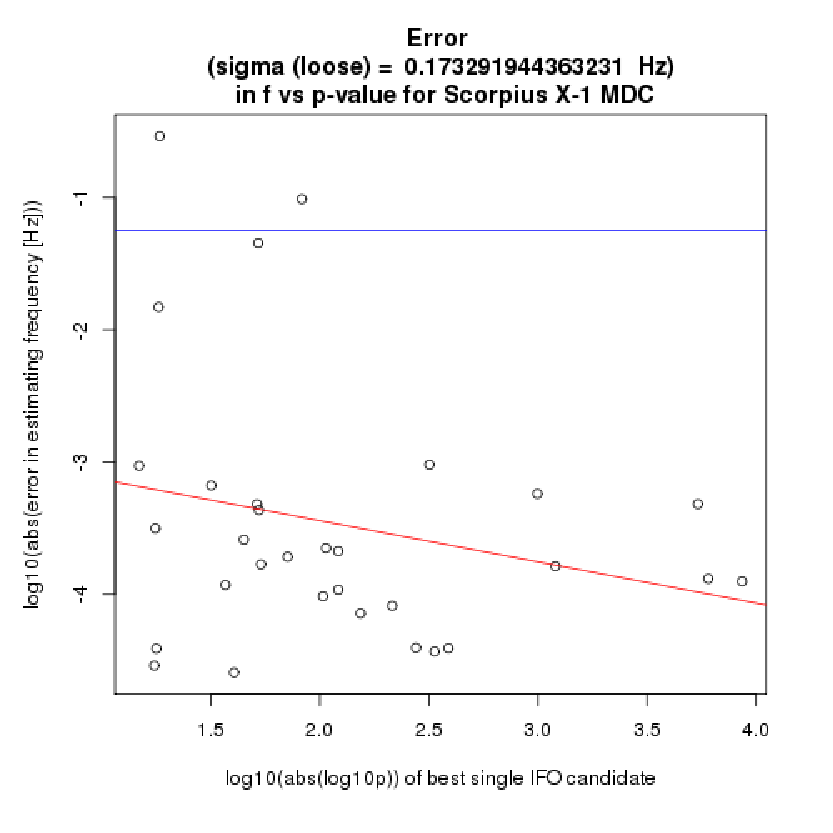
\includegraphics[width=0.3\paperwidth,height=0.2\paperheight]{ErrorF.eps}
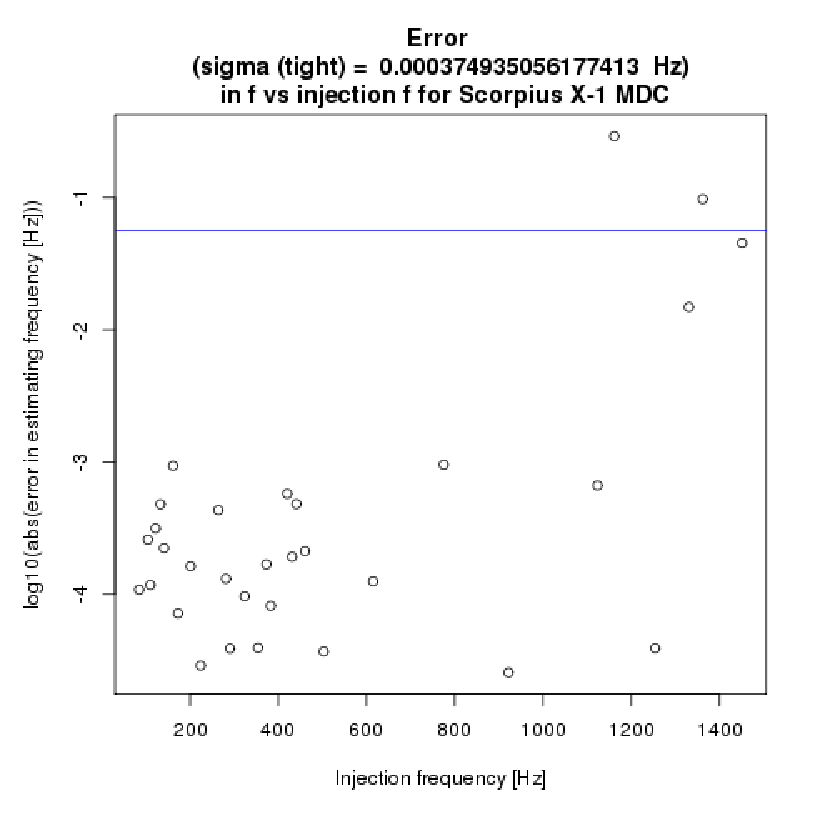
\includegraphics[width=0.3\paperwidth,height=0.2\paperheight]{ErrorFvsF.eps}
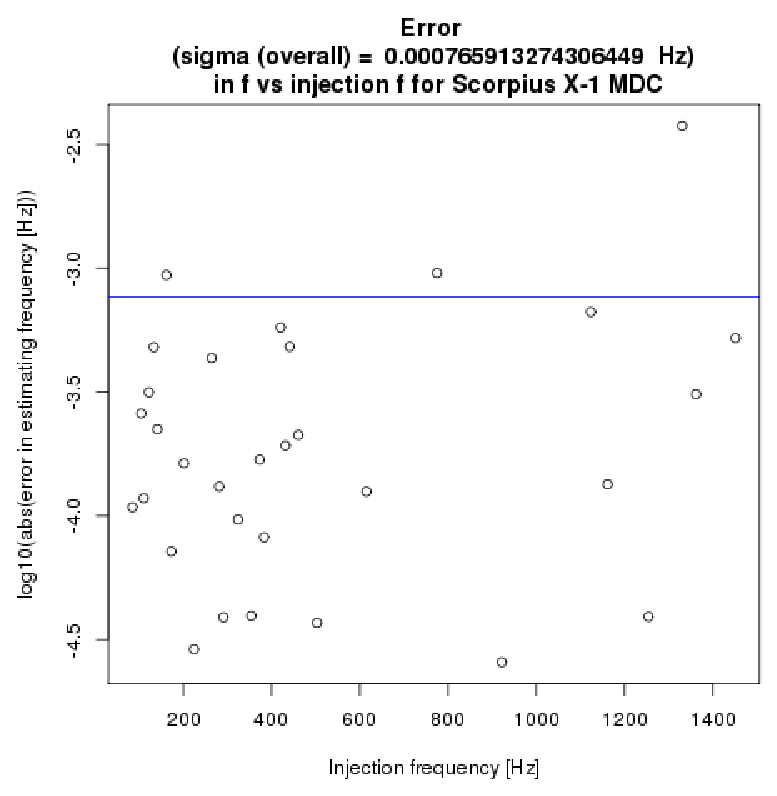
\includegraphics[width=0.6\paperwidth,height=0.4\paperheight]{plots/ErrorFvsF-overall.eps}
\caption{Parameter estimation: error in frequency as a function of recovered $p$-value (top left) and frequency (top right). A systematic, high error group can be seen, composed of four outliers in these graphs of the open data set. These defined the \textit{loose} fit category and prompted further investigation. The overall error vs frequency is shown at bottom after a rerun to fix a misconfiguration where inadequate data was read-in at high frequencies.
\label{fig:errorf}}
\end{center}
\end{figure}


\begin{figure}
\begin{center}
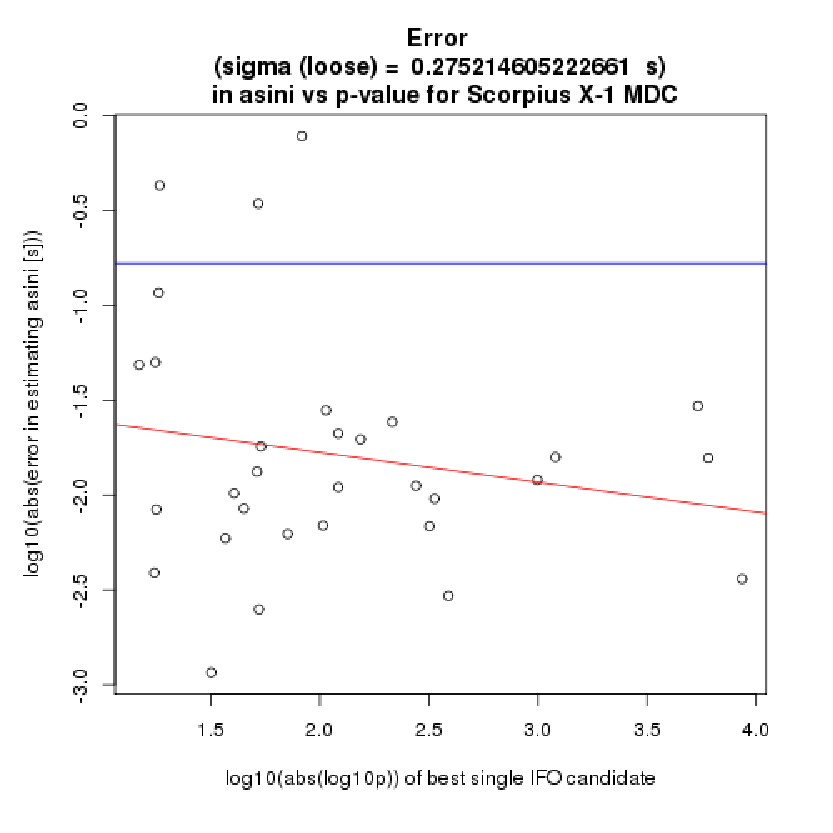
\includegraphics[width=0.3\paperwidth,height=0.2\paperheight]{ErrorAsini.eps}
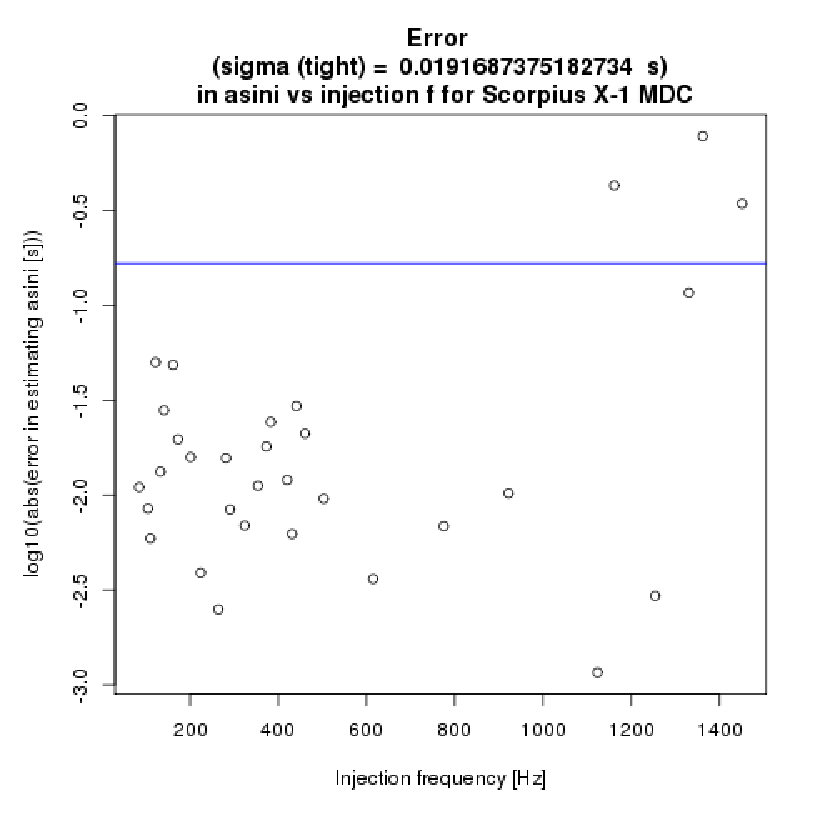
\includegraphics[width=0.3\paperwidth,height=0.2\paperheight]{ErrorAsinivsF.eps}
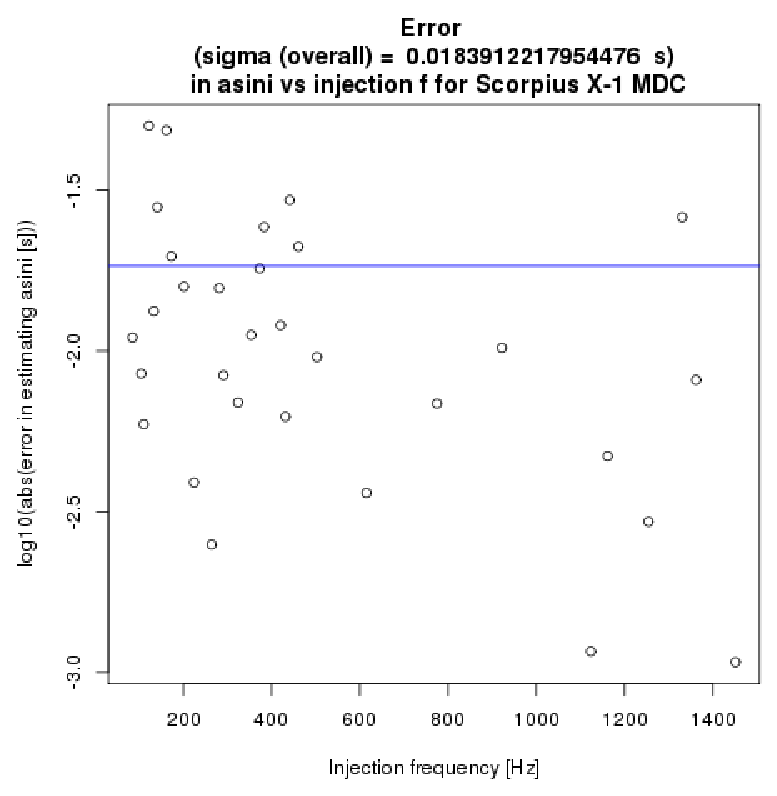
\includegraphics[width=0.6\paperwidth,height=0.4\paperheight]{plots/ErrorAsinivsF-overall.eps}
\caption{Parameter estimation: $a \sin\iota$ (projected semi-major axis; directly proportional to modulation depth for a given frequency and period) as a function of recovered $p$-value (top left) and frequency (top right). The overall error vs frequency is shown at bottom after a rerun to fix a misconfiguration where inadequate data was read-in at high frequencies.
Here the same \textit{loose} outliers suffer large errors.
\label{fig:errorasini}}
\end{center}
\end{figure}


\subsection{Upper Limits and Detection Efficiency}

Upper limits and detection efficiency were also calculated using data in the open pulsar set.

For detection efficiency, we calculated the $h$-effective for the 31 detected and 19 non-detected pulsars and found the average detection rate in bins according to $h$-effective. These bins were non-uniform in size due to the interest in finding the 95\% detection efficiency point despite the paucity of statistics (only 50 pulsars total). Binomial uncertainty was also calculated and subtracted, by bin. The 95\% level is very approximately about 3$\times 10^{-25}$ (again, without the corrective factors of 1.75 and 1.11) but is imprecise to judge using this method.

\begin{figure}
\begin{center}
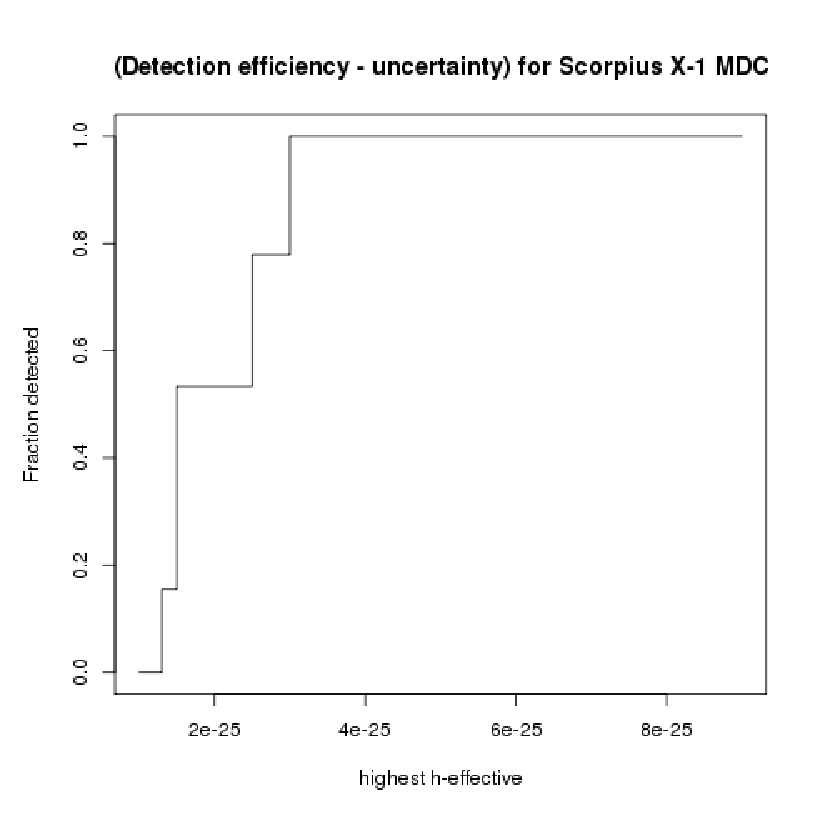
\includegraphics[width=0.3\paperwidth,height=0.2\paperheight]{detectionVsHeffective.eps}
\caption{ Open pulsar detection efficiency curve.
Because only 50 pulsars were in the open set, this curve is relatively-poorly defined -- the binning has been chosen to give the most accurate representation based on the chosen thresholds.
Binomial uncertainty was also calculated and subtracted, by bin. The 95\% level is very approximately about $3 \times 10^{-25}$ (again, without the corrective factors of 1.75 and 1.11) but is imprecise to judge using this method.
The curve is the worst case, equal to the efficiency minus the binomial uncertainty.
\label{fig:detectionvsheffective}}
\end{center}
\end{figure}


Consequently we plotted the distribution of recovered $h_0$ versus injected $h_0$-effective (the error of which is shown above, for detected pulsars)  in Figure~\ref{fig:hrecoveredvsheffectivefullul}. Further injection studies should show how this upper limit varies with frequency as injected $h_0$, but at the time of the MDC, we did not feel confident in extrapolating this relationship.

\begin{figure}
\begin{center}
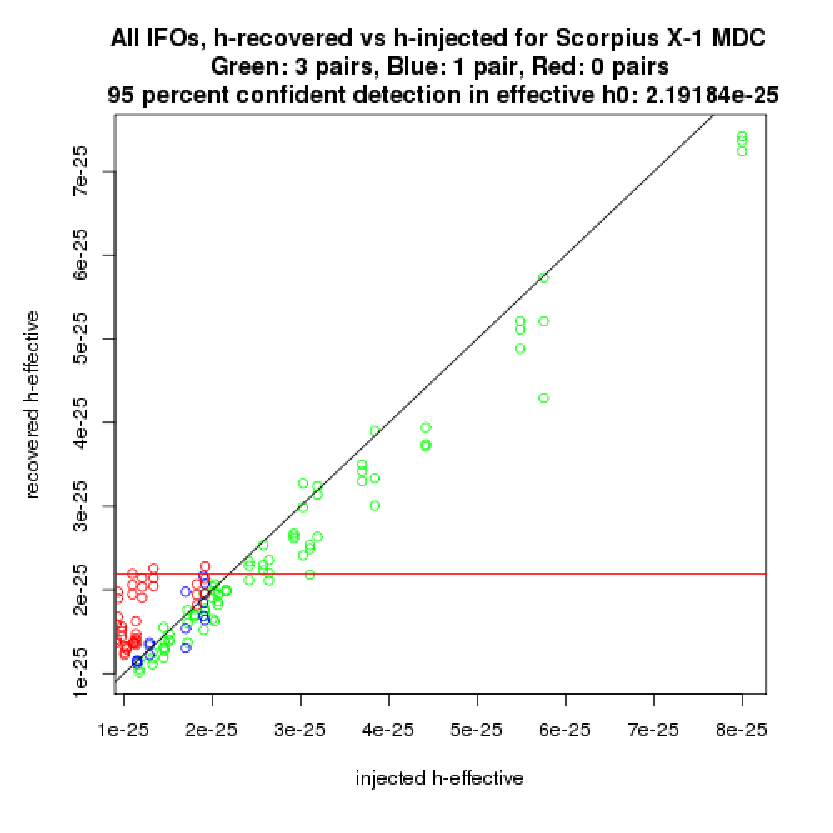
\includegraphics[width=0.3\paperwidth,height=0.2\paperheight]{HrecoveredVsHeffectiveFullUL.eps}
\caption{Detections and upper limit determination.
Depending on whether a injection was seen in three, one, or no detectors, it was assigned a color-coded circle and plotted in recovered strain versus effective circular strain injected.
Color-coding red pulsars as non-detected, blue as single pairwise detection, and green as triple pairwise detection, we identified a shelf of non-detected pulsars that was 95\% contained by an upper limit about $2.19 \times 10^{-25}$. This number, when corrected, yielded the upper limit of 1.74*1.11*$2.19 \times 10^{-25}$ = $4.23 \times 10^{-25}$ for TwoSpect. 
The unity-slope line is shown to ascertain whether a further rescaling factor was needed (it was: constant 1.11).
The zero-slope line is shown to indicate the ninety-five percent confidence upper limit.
\label{fig:hrecoveredvsheffectivefullul}}
\end{center}
\end{figure}


\subsection{$\cos \iota$ Ambiguity}

The cosine of the inclination angle of the pulsar, $\cos \iota$, casts an ambiguity over the determination of $h_0$. For TwoSpect, which assumes circular polarization, the true value of $h_0$ will indeed be as reported if $\cos \iota$ = 1, but will be greater if $\cos \iota$ is less (i.e., the gravitational wave is elliptically polarized). In the case of linear polarization, $h_0$ will be $2^{3/2}$ times larger than reported.

While an analytical calculation of the expectation value of the correction factor is easy, it will not easily take into account the circular bias of detected signals. That is, a pipeline will tend to see a slightly greater proportion of signals that are more circularly polarized, because the effective $h_0$ of those signals is greater. This ``circularizes" the correction factor in a way dependent on the detection efficiency of the pipeline and the assumed prior distribution of pulsars. Although the effect is relatively minor, we decided to simulate it because the size of the effect was unknown at the time.

In this simulation, 2 million pulsars were generated with $h_0$ between 3$\times 10^{-26}$ and 3$\times 10^{-24}$ (a rough guess at the scope of the MDC) with a distribution of 1/$h_0$.

We made a toy model of our detection efficiency, assuming no pulsars were detected below 1$\times 10^{-25}$ effective, all were above 3$\times 10^{-25}$, and the fraction detected was linear in $h_0$ between those values (Figure~\ref{fig:plotheffdisth0detectionefficiency200breaks}).

\begin{figure}
\begin{center}
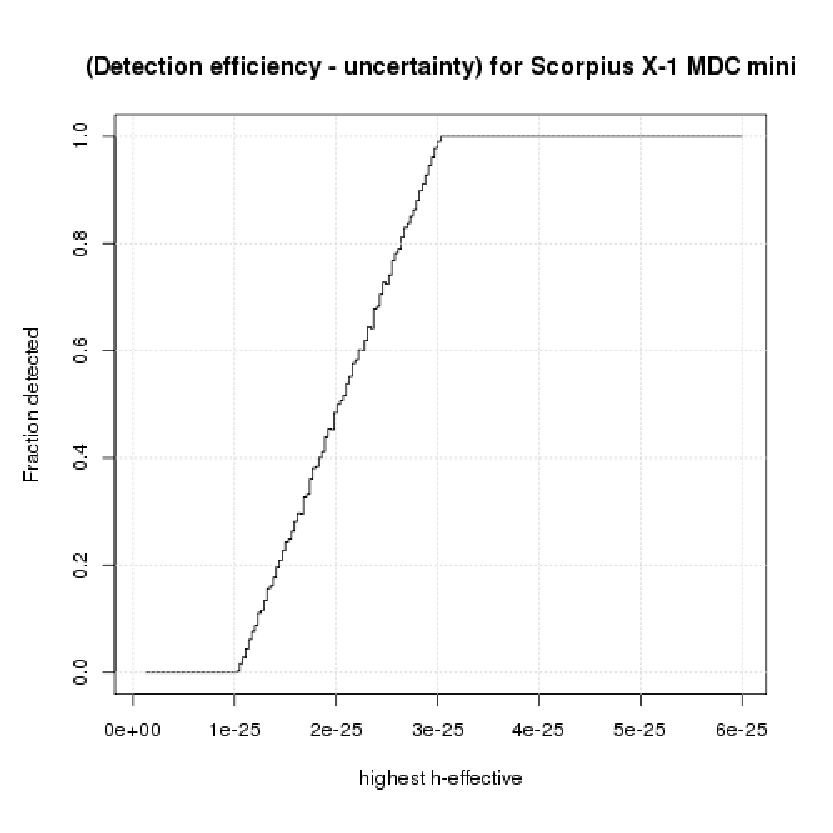
\includegraphics[width=0.3\paperwidth,height=0.2\paperheight]{PlotHeffDistH0DetectionEfficiency200breaks.eps}
\caption{ Simulated detection efficiency curve. Because the $\cos \iota$ ambiguity simulation require a priori model of detection efficiency, we described it simply. Here, no detections were claimed below $1\times 10^{-25}$, all were detected above $3\times 10^{-25}$, and the probability of detection rose uniformly on the intervening interval.
\label{fig:plotheffdisth0detectionefficiency200breaks}}
\end{center}
\end{figure}


Together with a uniform $\cos \iota$ distribution on [-1, 1], this led to a trapezoidal distribution of recovered, detected $h_0$ values with a curved lower (left) edge (Figure~\ref{fig:plotheffdisth0detected}).

\begin{figure}
\begin{center}
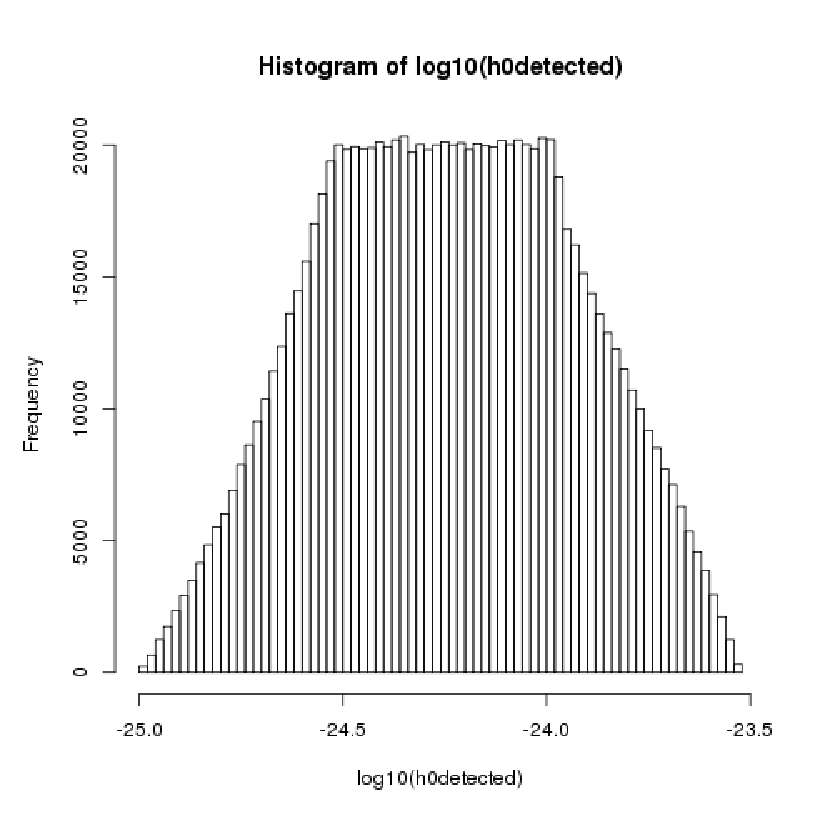
\includegraphics[width=0.3\paperwidth,height=0.2\paperheight]{PlotHEffDistH0Detected.eps}
\caption{Distribution of 2 million simulated stars, strain between $3\times 10^{-26}$ and $3\times 10^{-24}$ under a log-uniform distribution, following application of cos $\iota$ and detection efficiency cuts.
\label{fig:plotheffdisth0detected}}
\end{center}
\end{figure}


The upper end of the distribution (right side of the trapezoid, Figure~\ref{fig:plotheffdisth0detected}) was excluded because we are trying to find the average bijective mapping (slope) f: (detected $h_0$) $\rightarrow$ (true $h_0$), and including detected $h_0>$ 1$\times 10^{-24}$ meant that we were failing to see the complete injected $h_0$ space. There was f$^{-1}$: (true $h_0$) $\rightarrow$ (detected $h_0$), but not $f$. More plainly, suppose we looked at a detected $h_0$ reported as 1.5$\times 10^{-24}$, and that our average corrected factor had been calculated to be 2.5 (it was not) -- this would imply that the true $h_0$ was 3.75 $\times 10^{-24}$ -- but this would be outside the domain of the simulation, so there would be no way to check it. The analogous problem should not happen at the lower end of the distribution (left side of the trapezoid).

In turn, we looked for the relationship between the recovered $h_0$ of this ``detected" distribution and the corresponding original, true $h_0$. The slope would give us the conversion factor. The first attempt was to grid the {detected $h_0$}x{true $h_0$} space into 2D pixels. This was suggestive, and yielded the following regressed slope in Figure~\ref{fig:plotheffvsh0trueregressions}

\begin{figure}
\begin{center}
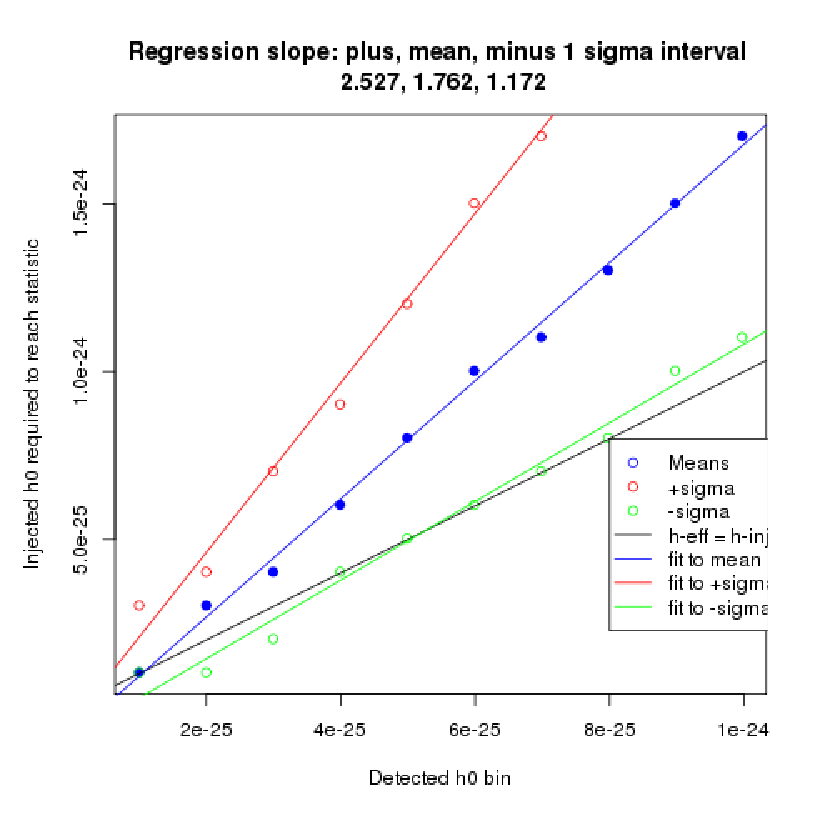
\includegraphics[width=0.3\paperwidth,height=0.2\paperheight]{PlotHeffVsH0TrueRegressions.eps}
\caption{Regression using grid. By binning the simulated stars on the true strain vs detected (recovered) strain plane, an accurate mean slope for the $\cos \iota$ correction was ascertained. It had to be modified downwards by the equivalent of one bin, to 1.74. However suggestive, the 1-$\sigma$ thresholds proved inaccurate, probably due to noise fluctuations.
\label{fig:plotheffvsh0trueregressions}}
\end{center}
\end{figure}


\begin{figure}
\begin{center}
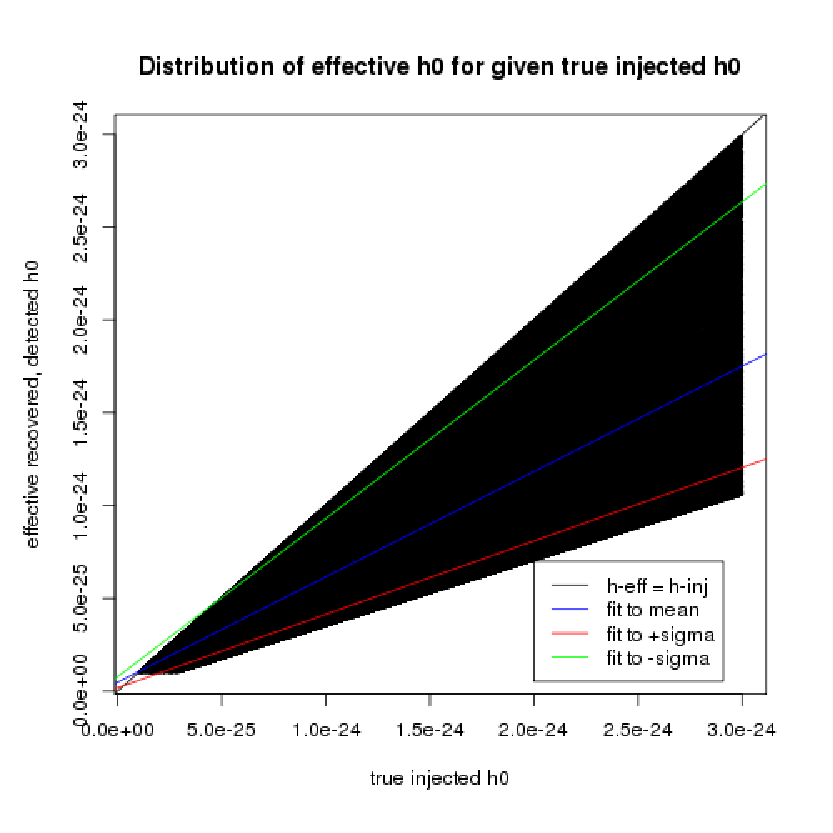
\includegraphics[width=0.3\paperwidth,height=0.2\paperheight]{PlotHEffVsH0TrueWithLines.eps}
\caption{Simulation with fit lines as given by the bin-method regression.
\label{fig:plotheffvsh0truewithlines}}
\end{center}
\end{figure}

There is a systematic bias in the grid method, both by one pixel (hence why the mean was adjusted downward to 1.74) and in the associated uncertainties. Plotting these uncertainties on the distribution of {detected $h_0$} vs {true $h_0$} shows how wide those error bars are, in Figure~\ref{fig:plotheffvsh0truewithlines}.


This bias in Figure~\ref{fig:plotheffvsh0truewithlines} is likely due to sampling: numerical fluctuations in the grid method made it unstable at the 2 million pulsar level, especially toward the high $h_0$ end of the distribution. Instead, we manually adjusted a $\pm \sigma$ until the CDF encompassed the appropriate 68\% confidence interval, finding a $\sigma$ in the slope of 0.37 with a mean slope of 1.74. The reason for the aforementioned restriction of the plot to $h$-effective $<$ 1$\times 10^{-24}$ can be seen in the distortion at levels above that in the following plot:

\begin{figure}
\begin{center}
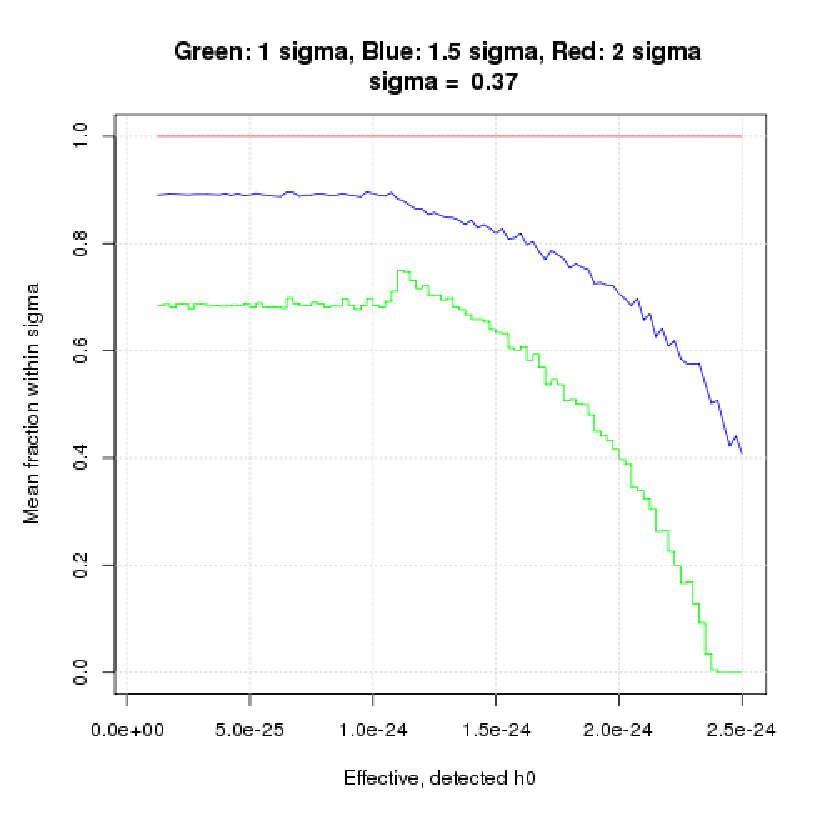
\includegraphics[width=0.3\paperwidth,height=0.2\paperheight]{PlotSigmaDiffVsH0Eff.eps}
\caption{Confidence intervals with final fit. After manual optimization of the cumulative distribution function, and constraint to the region with a full bijective mapping between injected and recovered strains (below $1 \times 10^{-24}$), a 1-$\sigma$ value of 0.37 in the slope was found to give accurate confidence intervals.
The reason for the aforementioned restriction of the plot to $h$-effective $<$ $1 \times 10^{-24}$ can be seen in the distortion at levels above that. The chosen $1.74 \pm 0.37 \sigma$, however, yielded the necessary correction factor. \label{fig:plotsigmadiffvsh0eff}
}
\end{center}
\end{figure}

The chosen $1.74 \pm 0.37 \sigma$, however, yielded the necessary correction factor.

Finally, we tested all of our calibration factors for $h_0$ with the associated confidence intervals and found the fraction of open data estimated $h_0$, f and asini within their 1 $\sigma$ error bars. The results were conservative:

$h_0$: 0.7741935 (77.4\%)
f: 0.7419355 (74.2\%)
asini: 0.6774194 (67.7\%)
Period: 1.00 (100\%) [n.b., we only tested one period, 68023.8259 s]

These error bars were then used without modification for claiming uncertainties on the closed pulsars.


%\end{frame}

\section{Summary of the MDC}
%\begin{frame}{Summary}
%\subsection{General summary for TwoSpect}

TwoSpect competed extremely effectively in the MDC.
Comparisons are the subject of a forthcoming paper, but for our own work, the author can report the following successes.

\subsection{Mock data challenge results}

Analyses of the MDC correctly recovered about two-thirds of the simulated stars:

\begin{itemize}
\item 34 of 50 closed (and 31 of 50 open) pulsars detected
\item $f$, $a \sin i$ and $h_0$ estimated
\item $4.23\times 10^{-25}$ strain UL in $4 \times 10^{-24}$ strain Hz$^{1/2}$ noise
\item with injections to refine UL, applicable to real data
\end{itemize}

One challenge in the transition to real data is that MDC used entirely Gaussian data.
Non-Gaussian test injections are the subject of Chapter~\ref{chap6}.
Although the distribution of $h_0$ values in the MDC was astrophysically optimistic, we gained knowledge about the transition from low- to high-SNR detections.
This MDC also validated our ability to recover orbital and GW parameters accurately, even for blinded simulations.

\subsection{Binary search summary beyond the MDC}
%\begin{itemize}
TwoSpect is well-suited to the Scorpius X-1 mock data challenge.
With this experience, the author is pursuing Scorpius X-1 (and J1751-305) searches in real data, as in Chapter~\ref{chap6}.
It is also believed that directed binary searches can be made more sensitive with straightforward changes (see Section~\ref{chap5_addendum}).
%\end{itemize}
%\begin{itemize}
In the near term, the author and the LIGO continuous waves group will direct TwoSpect and kindred binary searches toward promising targets such as LMXBs.
In the long term, this work will enhance all searches, the bridge of accreting binaries providing a firm link to electromagnetic astronomy as the age of gravitational wave astrophysics begins.
%\item TwoSpect binary searches -- directed, Sco X-1
%\end{itemize}

%\emph{Acknowledgments}


%Thanks to the American Physical Society for hosting this conference,
%as well as the University of Michigan, Evan Goetz for introducing
%TwoSpect, Keith Riles for guidance, and the LIGO Scientific Collaboration
%and National Science Foundation.
%\end{frame}
%\begin{frame}{Bibliography}
%\emph{References}
%\cite{Chakrabarty2003,GoetzThesis,GoetzTwoSpectMethods2011,PapaloizouPringle1978,Wagoner1984}
%\bibliographystyle{apsrev}
%\bibliography{bibliography}




%\end{frame}

\section{Plans for improvement}
%\begin{frame}{Plans for improvement}

TwoSpect presents a viable obtion for seeking continuous gravitational waves from neutron stars in binary systems, yet more sensitivity would reveal a richer sky.
Indeed, aLIGO designs and the Scorpius X-1 torque-balance limit do not guarantee detection in the coming generation of intereferometers.
Several improvements can thus be investigated.

\begin{itemize}
\item \emph{Coherently combine multiple interferometer outputs: }\\
Add complex Fourier coefficients (with phase corrections)\\
to create a multi-detector statistic (underway by Goetz)
\item \emph{Elliptical polarization:}\\
search antenna pattern weightings corresponding to\\
elliptical polarization -- better sensitivity
\item \emph{Orbital phase:}\\
Search over initial orbital phase by coherently combining\\
template and doubly Fourier-transformed data
\item \emph{Parameter space patterns:}\\
Exploiting patterns in the $R$-statistic parameter space\\
to improve search time, sensitivity, or both
\end{itemize}

%\end{frame}
%\begin{frame}{Polarization addendum}
%\subsection{Polarization addendum}

%Also: fastest known pulsar $f=$716 or 761 Hz(?)
%\end{frame}

%\begin{frame}{Coherent interferometer synthesis}
\subsection{Coherent interferometer synthesis}
Coherent interferometer synthesis for H1-L1-V1 is already well-underway by Goetz.
Data from multiple interferometers can be added in-phase for a putative signal model, and this technique already appears to be yielding improvements in detection efficiency.
To wit, the synthetized $h$ is given by Equation~\ref{TwoSpect_h_synth}:

\begin{equation}
h(f,t)=\Sigma_{j}\left(h_{j}(f,t)+\phi_{j}(f,\alpha,\delta)\right),
\label{TwoSpect_h_synth}
\end{equation}
\begin{equation}
\phi_{j}(f,\alpha,\delta)=2\pi fT_{j}(\alpha,\delta)+\phi_{0},
\label{TwoSpect_phase_synth}
\end{equation}

\noindent where $h_{j}(f,t)$ is the complex $h$ value in SFT for interferometer $j$, time $t$, frequency $j$ and
$\phi_{j}(f,\alpha,\delta)$ is the phase shift for right ascension $\alpha$,
declination $\delta$ 
(an overall phase shift $\phi_{0}$ factors out because
TwoSpect computes its test statistic from power, not the complex SFT coefficient).
Here,
$T_{j}(\alpha,\delta)$ is the time-of-flight delay between interferometers 
(projected on vector from $\alpha,\delta$).
Further investigations are forthcoming.

%\end{frame}

%\begin{frame}{Circular \& elliptical polarization}
\subsection{Circular \& elliptical polarization}


%\textbf{TwoSpect circular polarization assumption generalized}

The general formula for the polarization components of gravitation radiation is well-known.
The equation is stated (for instance, with $\Phi=2\phi$, in an earlier Scorpius X-1 search~\cite{AbbottScoX12007} or more recently in the TwoSpect all-sky search~\cite{GoetzTwoSpectResults2014}) in terms of two polarization components, $F_\times$ and $F_+$:

\begin{equation}
h(t)=h_{0} \left(F_{\times}(t,\alpha,\delta,\psi)\frac{1+\cos^{2}(\iota)}{2}\cos[\Phi(t)]+
F_{+}(t,\alpha,\delta,\psi)\cos(\iota)\sin[\Phi(t)]\right).
\label{TwoSpect_pol_effect}
\end{equation}

Presently, TwoSpect effectively searches only for circular polarization, making it most sensitive when $\cos \iota = 1$.
If antenna pattern weighting is adjusted to test for $F_\times$ and $F_+$ according to a general, elliptical polarization model, sensitivity to other values of $\cos \iota$ might hypothetically be enhanced.
It remains unclear whether this test would be sufficient by itself to remove the $\cos \iota$ ambiguity in estimated $h_0$ if a detection is obtained.

The current algorithm calculates pixel powers $P$ for SFT $n$, bin $k$:

\begin{equation}
\tilde{P}_{k}^{n}=\frac{F_{n}^{2}(P_{k}^{n}-<P_{k}>^{n})}{(<P_{k}>^{n})^{2}}\left[\Sigma_{n'}^{N}\frac{F_{n'}^{4}}{(<P_{k}>^{n'})^{2}}\right]^{-1},
\label{TwoSpect_pixel_powers}
\end{equation}
\begin{equation}
F^{2}(t,\alpha,\delta)=F_{\times}^{2}(t,\alpha,\delta)+F_{+}^{2}(t,\alpha,\delta),
\label{TwoSpect_pol_powers}
\end{equation}

\noindent where $F$ is antenna pattern polarization weighting.
Generalizing to elliptical polarization angle $\psi$ with weights $a,b$:

\begin{equation}
F^{2}(t,\alpha,\delta,\psi)=aF_{\times}^{2}(t,\alpha,\delta,\psi)+bF_{+}^{2}(t,\alpha,\delta,\psi)
\label{TwoSpect_elliptical_pol}
\end{equation}

%Better upper limits; inclination angle $\iota$?

%\end{frame}

%\begin{frame}{Orbital phase \& beyond}
\subsection{Orbital phase \& beyond}

%\textbf{Templates for orbital phase in the 2nd Fourier plane}
%\begin{itemize}
%\item Templates weight 2nd Fourier plane powers
%\item Possible: phase in 2nd Fourier bins
%\item Benefits: consistency between rows, binary orbital phase?
%\item Significant alteration to weighting $\rightarrow$ beyond R statistic
%\end{itemize}

Orbital phase is currently ignored.
Only power information in the 2nd Fourier plane is used to inform $R$-statistic templates.
Considerable information in the orbital phase is available.
Orbital phase should be more robust than gravitational wave phase against effects analogous to spin-wandering and timing glitches, in particular because the time resolution of orbital phase is relatively low.
Even for extremely short SFTs, a year-long science run produces only hundreds of thousands of SFTs, not billions of time samples.
Perhaps just an approximate orbital phase-match would be possible, by verifying that given time-frequency plane sinusoid powers (ignoring GW phase information) correspond to power in the 2nd Fourier (frequency prime-frequency) plane.
Such a change may be sufficient to warrant revising the $R$-statistic weighting scheme, but if successful would provide astrophysically compelling information about the time of ascension of a binary system.

\subsection{Parameter space patterns}
Other ideas abound. The idea of simulated annealing has arisen in personal communication (e.g., with Maria Alessandra Papa, Sam Finn and others), but it is generally though to address the wrong issues in our high-noise, weak-signal analyses. Also proposed there (and in personal communication with Ethan Obie Romero-Severson) were `hill-climbers' that could explore the parameter space until encountering one of the $X$-pattern arms. Again, due to the low SNR of our expected signals and the availability of computational resources being sufficient, this climbing strategy will probably not be necessary yet (one could imagine it being appropriate for a laptop looking for pulsars in third-generation detector data). It does, however, raise the question of the nature of the $X$-arms.

            How big are the $X$ patterns in the $R$ surface on the modulation depth versus frequency plane?
These $X$-patterns follow the lines $df = f_{\textup{signal}} \pm (f - f_\textup{signal})$, intersecting at $f_\textup{signal}$.

We expect the $X$ pattern to be where the template touches a peak or trough in the time-frequency plane, with an $R$ proportional to the peak in a way that is as the relative power of that bin compared the power in the whole sinusoid. 
Since the template touches only once per period, the ratio would be $T_{\textup{coh}} / P_{\textup{signal}}$. For Scorpius X-1 ($P = 68023.8259$ s), that would lead to ratios of roughly $0.026 \approx 1/38$ for 1800 s SFTs, $0.01 \approx 1/81$ for 840 s SFTs, and $0.0053 \approx 1/189$ for 360 s SFTs.

Yet in practice, as exemplified by pulsar 40 in the Mock Data Challenge, which used 360 s SFTs, the difference between the peak (correct template) $R$-value and the $X$-pattern arms was only a factor of 1/2 to 1/3.
This suggests that the `touch-at-one-point' model is oversimplified, and there is significant overlap still.
There would be a shearing process as $df$ deviates further from the true modulation depth, governed by the frequency bin resolution, $1/T_\textup{coh}$. 
For pulsar 40, $df = 0.046$ Hz, the amplitude of this modulation depth was only about $B = \left(2 \pi \textup{asini} f / P \right) \times \textup{coh} \approx $ 16 bins, with a period of 189 bins.
We could estimate the fractional power in the arms to then be $2 \pi / \cos^{-1} ((B-1) / B)$, or roughly $1/18$ for pulsar 40.
Taking the arccosine of $(B-2)/B$ instead yields roughly $1/12$.
This is closer to the 1/2 to 1/3 ratios observed in the analyses that than 1/189 predicted naively, although a proper study would require a closer look at the generation of TwoSpect \textit{exact templates}.

The deeper problem is that the wrong putative template and the true signal are both stationary are the same point in the time-frequency plane, stationary in the sense that their derivatives match:

\begin{equation}
\frac{df_\textup{true} (t)}{dt} = \frac{df_\textup{template}(t)}{dt} = 0.
\end{equation}

Understanding the $X$ structure more fully could inform future methods for maximum likelihood estimation on the $R$ statistic plane or, more likely, on the pushed-forward $p-value$ plane.
Theoretically, combining information from across the parameter space plane should create a strong signal.
This approach could parallel the deconvolution of point spread functions in optical imaging.
Although the deconvolution or Green's function would be different, this might also enhance the angular resolution when applied to spread on the right ascension, declination plane.
Constructing the deconvolved plane should in principle yield the same information as constructing a likelihood surface.
However, this approach needs to be tested.

An \textit{ansatz} of the point spread function made by summing a given pixel with the appropriate nearby diagonal neighbors was coded as a toy model in Python, with the resulting heatmap indeed being more square and less $X$-shaped near the injection template. However, the signal-to-noise ratio (mean subtracted number of standard deviations at peak) was reduced by a factor of about $7/4$. This suggests more research into an appropriate kernel would be needed for this method to be a success, although in principle the additional information in the $X$ arms should contribute information to a search. 

\subsection{Relevance to follow-up}

TwoSpect currently estimates $f$ and $a \sin i$ limited by the accuracy of its grid-spacing and some noise fluctuations. 
More refined grid spacing is possible in the event of a detection, although this has not been studied. 
Determining $h_0$ with greater accuracy is impossible without knowing $\cos \iota$ by another means. 
In the future, knowledge of gravitational wave polarization angle might inform $\cos \iota$, and coherent combinations of detector data within TwoSpect might reduce noise in detected LMXBs, as well as making quieter sources detectable. 

Coherent synthesis, elliptical polarization, and orbital phase improvements
need implementation, validation and testing.
It can be hoped that they will provide additional sensitivity for TwoSpect to yield more detections, and possibly to add new parameters to the list of what TwoSpect can estimate.
Although these enhancements will increase computational cost, we can also attempt to offload some of that cost to distributed computing, such at the CW group's Einstein@home project.
Together with quieter noise floor of advanced detectors, we may yet detect gravitational waves from neutron stars in binary systems.

Since data from the initial detectors exists now, it does not hurt to check to see whether, despite the astrophysical predictions, a signal might already be seen.
Chapter~\ref{chap6} presents this survey.

\section{Addendum}
\label{chap5_addendum}

%\end{frame}

%\begin{frame}{Scorpius X-1 parameters}
\subsection{Scorpius X-1 parameters}
\label{scox1_parameters}

Scorpius X-1 parameters are known to high accuracy, except for frequency~\cite{Galloway2014}.
The first LIGO search was published in 2007~\cite{AbbottScoX12007}.

\begin{itemize}
\item Distance: 9000 light-years (2.8 kpc)
\item Eccentricity: $<3\times10^{-3}$
\item Sky location: $\alpha$=16h19m55.1s, $\delta$=-15d38m24.9s
\item X-ray luminosity: 2.3 $\times10^{31}$W, 60000 $L_{Sol}$
%\item First LIGO search: Phys. Rev. D 76 (2007) 082001; gr-qc/0605028
%\item Torque-balance (Papaloizou and Pringle 1978) equation (Wagoner 1984),
%generally:
\end{itemize}

\textbf{Sco X-1 torque-balance limit (from X-rays)}~\cite{GoetzThesis}:
\begin{equation}
h_{0}=3\times10^{-26}\left(\frac{540\textup{Hz}}{f}\right)^{1/2}
\label{ScoX1_torque_bal}
\end{equation}

Note that Chakrabarty~\cite{Chakrabarty2003} has hypothesized the existence of an LMXB speed limit; given a fastest known millisecond pulsar of 716 Hz, this could imply that a search up to $2\nu \approx 2\times716 Hz = 1432$ Hz, plus a margin of error, should suffice to cover the astrophysical parameter space. 



%\end{frame}

        %---------------------------------

	%The following is an example of using the commands \textit{ref}
	%and \textit{label}. With these commands theorems, chapters,
	%sections and figurres can be labeld with names in the tex file
	%and then refered to by these names in later tex files. In
	%chapter~\ref{intro} we saw section~\ref{sample_section} or
	%theorem~\ref{sample_theorem}.

	%Lastly, here is how to include a figure. First generate an
	%encapsulated postscript file in xfig, adobe illustrator or
	%some other program. The specific commands are found in
	%\textit{chap2.tex}.

        %\begin{figure}[htb]
        %\centerline{ \epsfig{figure=sample.eps, 
        %height =  1.5 in}}
        %\caption{Sample Figure}
        %\label{sample_figure}
        %\end{figure}

